In the previous chapter, we have shown how S4BXI can be used to run high-level
APIs, and therefore run realistic applications in simulation. While our
validation experiments show a good accuracy of our method, the biggest drawback
of our model compared to state-of-the-art simulators is its performance. This
was even more noticeable in earlier versions of S4BXI: we managed to optimize
our model during the development of this chapter's work, allowing our
performance to get closer to SMPI's. In this chapter, we will explore ways to
improve the speed of simulation, using several network models, which will allow
us to dynamically switch at runtime between a slow and accurate model, and a
fast but less accurate one. This is useful to model precisely a region of
interest of the simulation, while modeling other parts coarsely.

We will start by motivating our choice of models in
Section~\ref{sec:6_model_change:simgrid}, and show how these two models are used
in Section~\ref{sec:6_model_change:division}. Then we will detail the technical
developments that are required to implement model changes in
sections~\ref{sec:6_model_change:model_change_arch},~\ref{sec:6_model_change:interception}
and~\ref{sec:6_model_change:coherency}. Additionally, we will explain how we can
make model changes more flexible by tracking asynchronous operations in
Section~\ref{sec:6_model_change:request_tracking}. Finally, we will present our
experimental results in Section~\ref{sec:6_model_change:experiments}, and
conclude in Section~\ref{sec:6_model_change:conclusion}.

\section{Design choices}

\subsection{Two network models over SimGrid}
\label{sec:6_model_change:simgrid}

Since S4BXI is based on SimGrid, we chose to support the following network
models: Atos's implementation of OpenMPI on top of S4BXI, and SMPI. Using SMPI
as a second model is very convenient from a technical perspective: since both
models rely on SimGrid, they naturally share a common source of truth for the
simulated time, they both use SimGrid's Actor system. If we wanted to support
different state-of-the-art models, for example SystemC emulators or abstract
LogGOPS simulators, most of our methodology would work the same way, except that
a significant development effort would be required to make the architecture of
the simulators compatible. For example, it would require synchronizing the
simulated time in all models, making sure the scheduling of actors performed by
SimGrid is compatible with the other simulators, etc.

\subsection{Different ideas to share the network loads}
\label{sec:6_model_change:division}

Before we explain how SMPI is used in an otherwise ``S4BXI'' simulation, we need
to discuss the way our two models are going to be used. There are essentially
two ways of dividing our usage of the simulators: either ``spatially'' or
``temporally''.

A spatial division is pertinent when some nodes of the cluster are more
interesting to study than others (for example the ``root'' node in a collective
operation with a ``tree'' implementation). In this case, the other nodes would
use SMPI to have a better performance, and the selected node(s) would use
OpenMPI over S4BXI to have a better accuracy. Such an execution is depicted on
Figure~\ref{fig:6_model_change:spatial}, with a simplistic cluster of three
nodes connected to a single switch.

\begin{figure}[!ht]
    \centering
    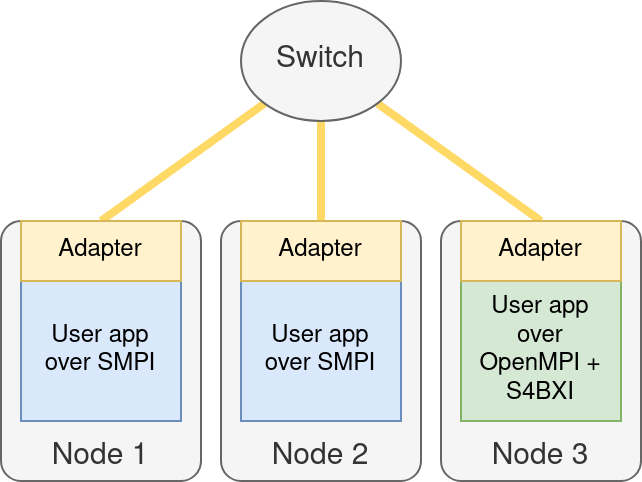
\includegraphics[width=0.5\textwidth]{6_model_change/spatial.png}
    \caption{Spatial distribution of the network models}
    \label{fig:6_model_change:spatial}
\end{figure}

This approach has two main downsides: first, it is not always trivial to select
which nodes should be modeled with high accuracy, and which ones should be
modeled in a more performant way. It would be particularly hard and impractical
to express it manually in user applications' code, and making the decision
automatically would require having a very good knowledge of the different
algorithms for collective operations used in MPI, in order to make a heuristic
more efficient than deciding at random. Second, allowing nodes that run
different models to communicate together is a significant challenge, which would
require intrusive modifications in each model's code (S4BXI and SMPI) in order
to have ``adapters'' between the two models (which are shown on
Figure~\ref{fig:6_model_change:spatial}). Indeed, while both models rely on
SimGrid's Mailbox system to communicate, these Mailboxes currently use different
names, and the format of data exchanged through them is very different.
Additionally, collective operations use different algorithms when performed in
SMPI and OpenMPI over S4BXI, which results in a different set of point-to-point
communications. Reconciling these two implementations of collectives would be a
very significant challenge if we wanted to use different models on different
machines at the same simulated time.

\begin{figure}[!ht]
    \centering
    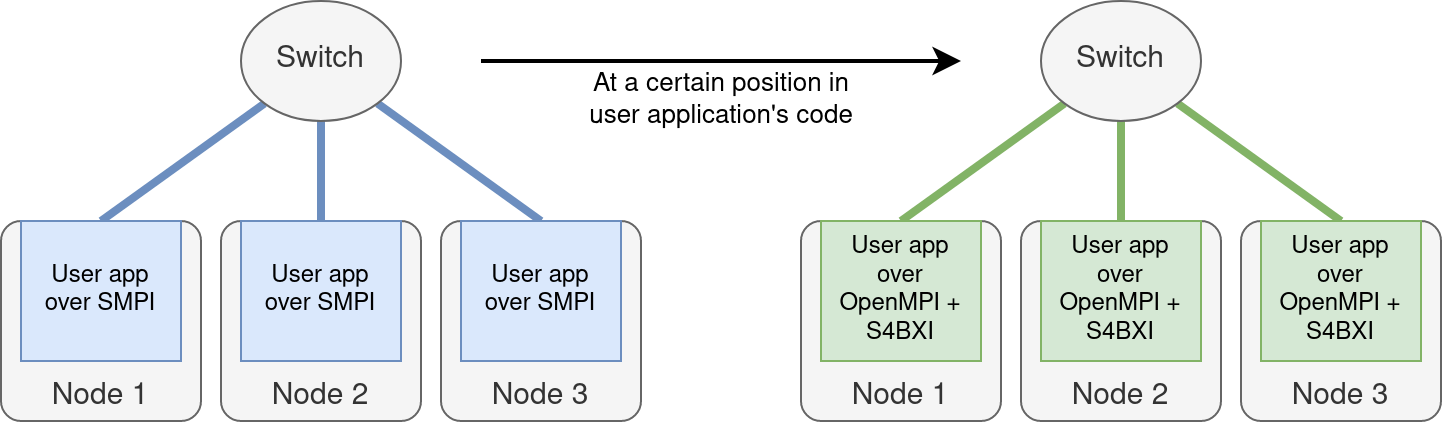
\includegraphics[width=1\textwidth]{6_model_change/temporal.png}
    \caption{Temporal distribution of the network models}
    \label{fig:6_model_change:temporal}
\end{figure}

On the other hand, a temporal division means that instead of focusing our study
on a specific set of nodes, we focus on certain ``phases'' of users'
applications. This idea leverages the fact that HPC applications typically have
long execution times, with different workloads in different phases of the
application. For example, an application could have an initialization phase,
then intense computation, and finally a phase to collect the results and make
statistics about the execution. In such a scenario, having a precise model of
the first and last phases is usually not very important, and it would be
desirable to focus on the computational phase with our precise model. An example
of this idea is depicted on Figure~\ref{fig:6_model_change:temporal}, with the
same three-nodes cluster, and two different phases: a first one which we
simulate quickly, in order to focus on the second one with our more accurate
model. This solution has the advantage that at every moment all nodes use the
same model, therefore there is no need for ``adapters'' between models. It is
also easier to decide when to switch models: a superficial knowledge of
applications is usually enough to have a good idea of the different phases they
go through. Therefore, it is relatively easy to manually add a line of code in
the application in the places where a model change should occur.

For this reason, in our study we will only implement a temporal division of the
usage of our two models.

\section{Architecture changes in S4BXI to support SMPI}
\label{sec:6_model_change:model_change_arch}

\subsubsection{Separation of S4BXI components}

In order to enable dynamic model changes during a simulation, we added a
component to S4BXI, called ``MPI middleware'', which manages our two MPI models
(OpenMPI over S4BXI and SMPI). It is important to note that even though our MPI
middleware is part of S4BXI, its function is very different from our Portals
implementation in S4BXI. Indeed, even though our simulator consists of only one
codebase, three functions must be distinguished:

\begin{enumerate}
    \item\label{item:6_model_change:portals} S4BXI exposes the Portals API to
    any code that links against it, implementing Portals using SimGrid's Mailbox
    system to exchange data, as presented in Chapter~\ref{chap:low_level}.
    \item\label{item:6_model_change:s4bximain} It also provides a set of
    utilities to run unmodified user code, using a method heavily inspired by
    SMPI (with on-disk copies of libraries and ``dlopen'' calls), which was also
    presented in Chapter~\ref{chap:low_level} (and extended in
    Chapter~\ref{chap:high_level} to support MPI simulation).
    \item\label{item:6_model_change:middleware} Finally, it features an MPI
    middleware, which exposes the MPI API, and implements mechanisms to manage
    two underlying implementations of MPI, which we detail in this chapter.
\end{enumerate}

\subsubsection{A note regarding software design}

For our purpose, having all three features in the same codebase allowed us to
prototype a working simulator quickly, but in order to make a full product out
of this simulator it would be advisable to split the code into well-defined
modules with proper interfaces. In particular,
features~\ref{item:6_model_change:portals}
and~\ref{item:6_model_change:s4bximain} are also part of a single codebase in
SMPI: while our Feature~\ref{item:6_model_change:portals} is completely
different from SMPI's counterpart, since SMPI implements MPI instead of Portals,
there are many similarities between S4BXI's and SMPI's
Feature~\ref{item:6_model_change:s4bximain}. Having this feature better isolated
from the rest of SMPI would have allowed us to re-use it instead of
re-implementing most of it. Indeed, the mechanisms used to isolate simulated
processes are independent of the API that is implemented by the simulator.
Consequently, it would be beneficial to make it a re-usable component of SimGrid
(instead of being a part of SMPI). Better decoupling would thus be desirable, as
discussed informally with SimGrid's development team, but it has not been done
during this PhD. It could also be a good occasion to evaluate different
techniques to isolate simulated processes: for example the project Remote
SimGrid\footnote{\url{https://framagit.org/simgrid/remote-simgrid/}} proposes an
experimental methodology which uses distinct processes that communicate with a
central SimGrid ``server'' using a custom BTL in OpenMPI. This type of approach
could be used in a shared component by both S4BXI and SMPI.

\section{Redirecting MPI calls using S4BXI's middleware}
\label{sec:6_model_change:interception}

In order to switch dynamically between two MPI implementations, we need to be
able to intercept calls to the MPI API. In order to do this, we re-use the same
method that we presented in Chapter~\ref{chap:low_level} in order to intercept
calls to \inline{sleep}, \inline{gettimeofday}, etc.: we inject an additional
header in users' applications, which uses C-style macros (\inline{#define}) to
redirect MPI calls to our functions. A few examples of these macros are given on
Figure~\ref{fig:6_model_change:middleware_macros} (passing the file and line of
the MPI call to our function is only useful to our logging system, which helped
us debug our middleware more easily).

\begin{figure}[!ht]
    \lstinputlisting[basicstyle=\ttfamily\small,frame=bt,language=C]{6_model_change/middleware_macros.h}
    \caption{Example macros to intercept MPI calls}
    \label{fig:6_model_change:middleware_macros}
\end{figure}

\begin{figure}[!b]
    \lstinputlisting[
        basicstyle=\ttfamily\scriptsize,
        frame=bt,
        language=C++,
        literate={.}{{$\nearrow$}}1 {,}{{$\nwarrow$}}1
    ]{6_model_change/smpi_request_null.cpp}
    \caption{Example implementation of a ``constant'' in our middleware}
    \label{fig:6_model_change:smpi_request_null}
\end{figure}

Now that calls are redirected to our middleware, we need a way to forward them
to the correct implementation (OpenMPI over S4BXI or SMPI). To achieve this, we
need our middleware to store pointers to every symbol of both MPI
implementations, so that we can decide which one to use at runtime. Of course,
we cannot rely on functions' names since they are the same in both libraries.
To get these pointers, we use the \inline{dlopen} and \inline{dlsym} functions
on both SMPI and OpenMPI at the start of the simulation. It is important to note
that even though SMPI is instantiated only once, each simulated process has its
own copy of OpenMPI (as presented in
Section~\ref{sec:5_high_level:relinkage_of_libs}), which means that the pointers
to MPI symbols must be specific to each simulated process (at least the OpenMPI
ones). It is also worth mentioning that even though most symbols we need to
intercept are functions, we also need to support constants which can have
different values in different implementations, such as \inline{MPI_REQUEST_NULL}
for example. This means that even though these symbols need to appear constant
to each MPI implementation, from our middleware's perspective they must be
implemented as functions which can return two different values, as illustrated
for \inline{S4BXI_MPI_REQUEST_NULL} on
Figure~\ref{fig:6_model_change:smpi_request_null}.

\begin{figure}[!b]
    \centering
    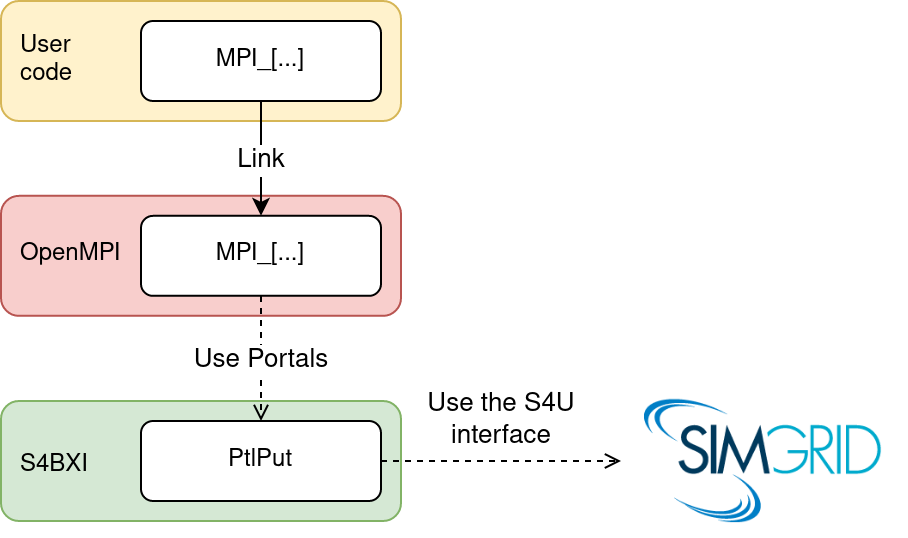
\includegraphics[width=0.65\textwidth]{6_model_change/regular_symbols.png}
    \caption{Execution of an MPI call, before adding our middleware}
    \label{fig:6_model_change:regular_symbols}
\end{figure}

\begin{figure}[!b]
    \centering
    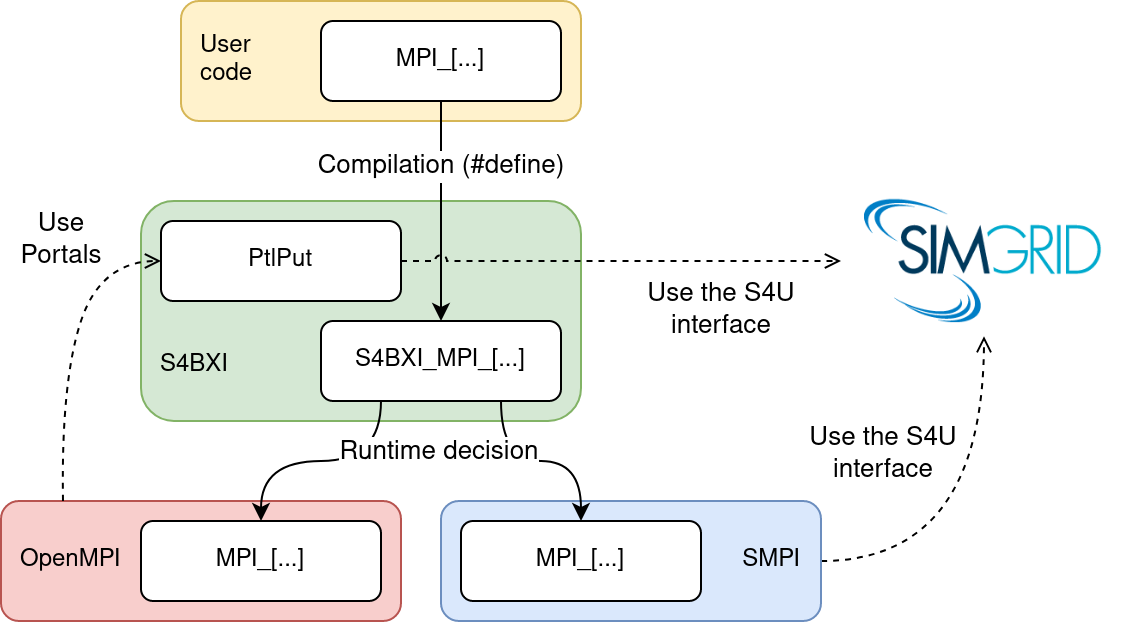
\includegraphics[width=0.75\textwidth]{6_model_change/intercept_symbols.png}
    \caption{Execution of an MPI call, after adding our middleware}
    \label{fig:6_model_change:intercept_symbols}
\end{figure}

Finally, we need to be able to instantiate SMPI from S4BXI. While this does not
seem to be the most difficult part, it still required some development effort:
indeed, SMPI expects to be started from the \inline{smpirun} or
\inline{smpireplay} binaries, and there is no out-of-box way of setting it up
programmatically. In particular, a few symbols we need were not originally
public in the SimGrid library, which made it impossible to link against them in
S4BXI. Thankfully, SimGrid's development team was kind enough to make a patch to
SMPI to allow us to use these symbols. Additionally, to use some of the
functions that are needed to set up SMPI, we have to import a few header files
directly from SimGrid's sources, because they are not part of the public headers
that are installed with each release of SimGrid. In the end, thanks to the
cooperation of SimGrid's development team, and thanks to the clean architecture
of SMPI's code, we are able to instantiate SMPI's model programmatically from
S4BXI, without having to patch SimGrid (even though it is not an officially
supported use-case of SMPI).

Thanks to these three steps, our middleware is able to instantiate SMPI and
extract symbols from both SMPI implementations at the start of simulations,
which allows us to intercept functions calls at runtime and forward them to
either implementation, based on a configuration parameter of S4BXI. From a
practical standpoint, switching from one MPI implementation to the other is
achieved through a call to S4BXI's \inline{s4bxi_use_smpi_implem} function,
which needs to be performed by all simulated processes. Therefore, it is the
responsibility of the application's developer to ensure that all MPI ranks
change their MPI model at the same point in the application. In particular, it
is important for all sides of each communication to be performed in the same
model: for example, a ``send'' and a ``receive'' must be performed with the same
MPI implementation on both processes involved. The initial implementation to use
when the simulation starts can be configured using the environment variable
\inline{S4BXI_SMPI_IMPLEM}. The resulting control flow of an MPI call is
depicted on Figure~\ref{fig:6_model_change:intercept_symbols}. This figure can
be compared to the method of Chapter~\ref{chap:high_level} which does not
involve a middleware, and is depicted on
Figure~\ref{fig:6_model_change:regular_symbols}.

\section{Maintaining MPI's internal coherency}
\label{sec:6_model_change:coherency}

In the development of our middleware, there is a difficulty that needs to be
considered: we cannot simply redirect MPI calls to the currently used
implementation, otherwise any switch between the MPI models would cause crashes
in our simulation. The reason is that some function calls must be forwarded to
both implementations instead of just one, in order to maintain a consistent
state in both implementations of MPI: the most obvious examples are
\inline{MPI_Init} and \inline{MPI_Finalize}, which need to be called in both
implementations in order to set them up correctly. Furthermore, the state of
both implementations needs to be kept in sync in other places too: in MPI, users
can create their own communicators, by splitting the global communicator
(\inline{MPI_COMM_WORLD}, which holds every process of the current job), which
is useful to perform collective operations on a subset of the MPI ranks in the
current job. Similarly, users can create their own datatypes, from combinations
of the basic types that MPI provides, in order to simplify the transmission of
message containing custom data structures. These communicators and datatypes are
opaque types from the point of view of the user's application: they are only
manipulated through MPI calls, and therefore their internal structure is left to
the implementation. As a consequence, the internal data structure created in one
MPI implementation cannot be used in the other, but we still need the datatypes
and communicators that are created in one model to be usable in the other.

\begin{figure}[!b]
    \lstinputlisting[basicstyle=\ttfamily\small,frame=bt,language=C++]{6_model_change/BxiMpiComm.hpp}
    \caption{\inline{BxiMpiComm}'s class declaration}
    \label{fig:6_model_change:BxiMpiComm}
\end{figure}

The simplest way to achieve this is again to call both implementations
regardless of the current model: when an application creates or modifies a
communicator or a datatype, we forward these modifications to both
implementations. To appropriately dispatch these modifications, we add wrappers
around communicators and datatypes, called respectively \inline{BxiMpiComm} and
\inline{BxiMpiDatatype}. Their function will be explained by using communicators
as an example, even though datatypes work in a very similar way. The declaration
of \inline{BxiMpiComm} is shown on Figure~\ref{fig:6_model_change:BxiMpiComm}.

\begin{figure}[!b]
    \centering
    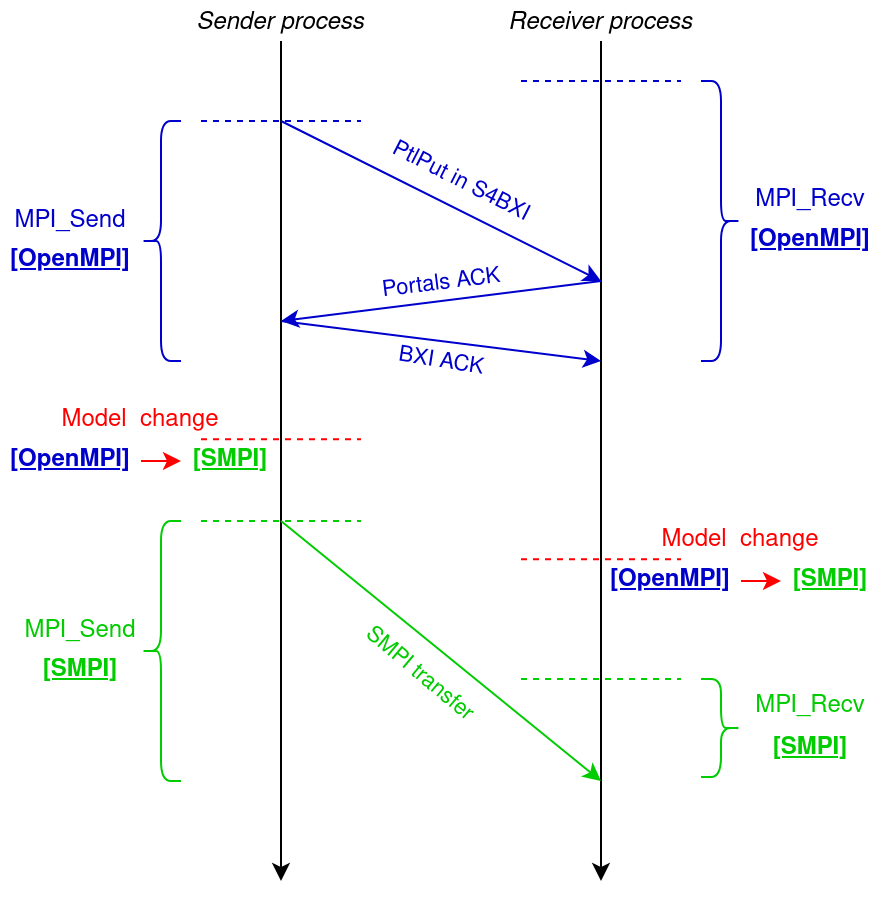
\includegraphics[width=0.7\textwidth]{6_model_change/sync_operations_model_change.png}
    \caption{Sequence diagram for two MPI data exchanges, after adding our middleware}
    \label{fig:6_model_change:sync_operations}
\end{figure}

As we can see on the figure, our wrapper holds a reference to the implementation
of the current communicator in both models (Atos's OpenMPI and SMPI). The three
utility functions are used to either fetch a specific implementation
(\inline{bull_comm} and \inline{smpi_comm}), or get the correct one according to
the current configuration (which model is currently being used), with
\inline{implem_comm}. This last function also needs to handle specific
communicators, such as \inline{MPI_COMM_WORLD} and \inline{MPI_COMM_SELF}.
Indeed, these communicators are not user-created: \inline{MPI_COMM_WORLD}
automatically holds all MPI ranks of the current job, and \inline{MPI_COMM_SELF}
only contains the current process. It is worth noting that even though C and C++
are statically typed languages, we can manipulate SMPI communicators, Atos
communicators, and S4BXI communicator wrappers using the type \inline{MPI_Comm}
every time, because in all three cases an \inline{MPI_Comm} is an opaque type
corresponding to a pointer, and therefore it always has the same size.
Unfortunately, we do not have any way to keep type safety here without making
many modifications in SMPI or Atos's MPI, because both models implement the same
specification (MPI), and therefore they have to use the same names for
communicators and datatypes. As a consequence, we have to be very careful when
casting an \inline{MPI_Comm} to any of the three implementations (two models
plus our wrappers), since we are losing type safety by using one general type to
store pointers to more specific structures. Thankfully this is completely
transparent to user applications, as casts only appear in our middleware where
extra care has to be taken to avoid errors when casting types. For example, in
\inline{implem_comm}, the parameter \inline{original} comes from the
application, and therefore it hides a pointer to a \inline{BxiMpiComm}, whereas
the return value will hide a pointer to an \inline{MPI_Comm} from either Atos's
implementation or SMPI. \inline{bull_comm} and \inline{smpi_comm} also take the
same parameter, but they always return the same kind of \inline{MPI_Comm}.

An example of communications using our middleware is depicted on
Figure~\ref{fig:6_model_change:sync_operations}, where a sender process will
first transmit a message to the receiver process in the OpenMPI over S4BXI
implementation of MPI, and then a second message in the SMPI implementation. The
associated code is shown on Figure~\ref{fig:6_model_change:sync_operations_code}
We can see that the first transfer uses Portals, which is implemented by S4BXI,
whereas the second one is simply handled by SMPI with a more simple model. We
can also see that it does not matter if model changes do not occur at the exact
same simulated time in all MPI ranks, as long as both sides of each
communication (a synchronous send and receive here) are performed in the same
model.

\begin{figure}[!b]
    \lstinputlisting[basicstyle=\ttfamily\scriptsize,frame=bt,language=C,aboveskip=0pt,belowskip=0pt]{6_model_change/example_sequence.c}
    \caption{Code for two MPI data exchanges, after adding our middleware}
    \label{fig:6_model_change:sync_operations_code}
\end{figure}

\section{Making model changes more lenient}
\label{sec:6_model_change:request_tracking}

At this point, our method to switch models dynamically works in most cases, but
there are conditions under which model changes could cause a crash: asynchronous
operations. For example, if an application starts an operation in Atos's MPI,
then switches to SMPI, and finally waits for the completion of the request, an
error would occur at runtime. Indeed, calling SMPI's \inline{MPI_Wait} primitive
with an \inline{MPI_Request} created by Atos's implementation is obviously
erroneous (as requests are also an opaque type with very different underlying
implementations). This specific example is depicted on
Figure~\ref{fig:6_model_change:request_tracking_example}.

\begin{figure}[!ht]
    \centering
    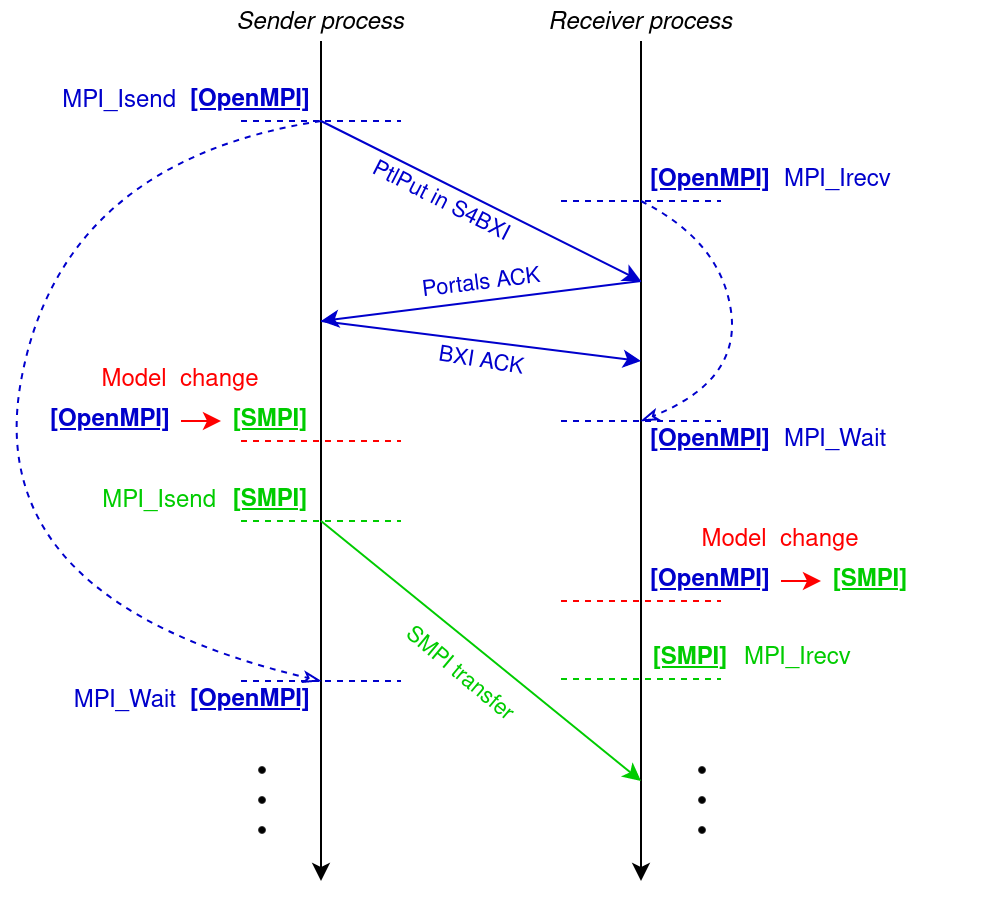
\includegraphics[width=0.7\textwidth]{6_model_change/request_tracking.png}
    \caption{Illustration of problematic asynchronous operations: sender process waits on an OpenMPI request after switching to the SMPI model}
    \label{fig:6_model_change:request_tracking_example}
\end{figure}

In order to handle this issue, and allow users to switch models at nearly any
point in the execution of their application, we keep track of  asynchronous
requests created by the user. In this context a request is a broad concept, as
it could represent any asynchronous operation: a ``send'', a ``receive'', a full
collective communication, etc. We keep track of all asynchronous requests
created in the SMPI implementation of MPI and to complete an asynchronous
request we check the model in which the request was created, i.e. whether it is
tracked as an SMPI request or not, and switch to the adequate model to handle
the completion event.

The way we implement it is with a C++ \inline{unorder_set}, in which we store a
pointer to every \inline{MPI_Request} that is created in the SMPI implementation
of MPI. Then, each time a request is queried (by \inline{MPI_Wait},
\inline{MPI_Test}, etc.), instead of checking the model in use for the current
Actor globally, we look for the request in our \inline{unordered_set}: if we
find it, then it is an SMPI one, and therefore we must use the SMPI variant of
the requested primitive, even if the user switched to OpenMPI in the meantime.
Conversely, if the request is not found, then it is an OpenMPI one, and we must
use Atos's primitive. If we go back to our example on
Figure~\ref{fig:6_model_change:request_tracking_example}, with our asynchronous
request tracking, the sender process will use OpenMPI's \inline{MPI_Wait} on the
request created by the first \inline{MPI_Isend} even though the application
switched to SMPI in the meantime.

This new addition to the middleware implies that the change of model is no
longer happening all in one go, when the user requests it, since a few
communications are still on their way and will be handled in the model
previously in use. This could be perceived as a problem for the interpretation
of the simulation result, as the two models are mixed, but events that are
interpreted in the ``previous'' model are not  causing any communication: they
are only primitives that test the completion of requests. Consequently, these
events interpreted in the ``wrong model'' are not going to cause major
discrepancy in the accuracy or speed of the simulation. Additionally, in
realistic cases it is likely that users will switch model in places where few
asynchronous requests are pending, therefore very few MPI calls will use the
``previous'' model.

Finally, a concern we had while implementing this feature regards performance:
when using SMPI, each time a primitive takes a request as a parameter, our
\inline{unordered_set} of pointer will be traversed to determine the model to
use (in the case of Atos's OpenMPI, the \inline{unordered_set} would be empty
most of the time so the problem is not as significant). We feared that this
might be costly in terms of CPU time, which is why we tested different
structures to keep track of requests, and concluded that the
\inline{unordered_set} is the most performant. In the end, across the
applications we tested, the difference in performance between keeping track of
SMPI requests or not ends up being negligible, therefore we did not add an
option to turn off this feature when using S4BXI's MPI middleware.

\section{Experimental results}
\label{sec:6_model_change:experiments}

In order to test our model changes, we used three applications: OSU
micro-benchmarks, Quicksilver, and HPL. Since HPL gives very similar results in
simulations that are completely in SMPI or completely in OpenMPI over S4BXI, we
did not obtain any noticeable difference in performance by adding model changes,
and therefore this section will only present our results with OSU
micro-benchmarks and Quicksilver.

\subsection{OSU micro-benchmarks}

\begin{figure}[!h]
    \centering
    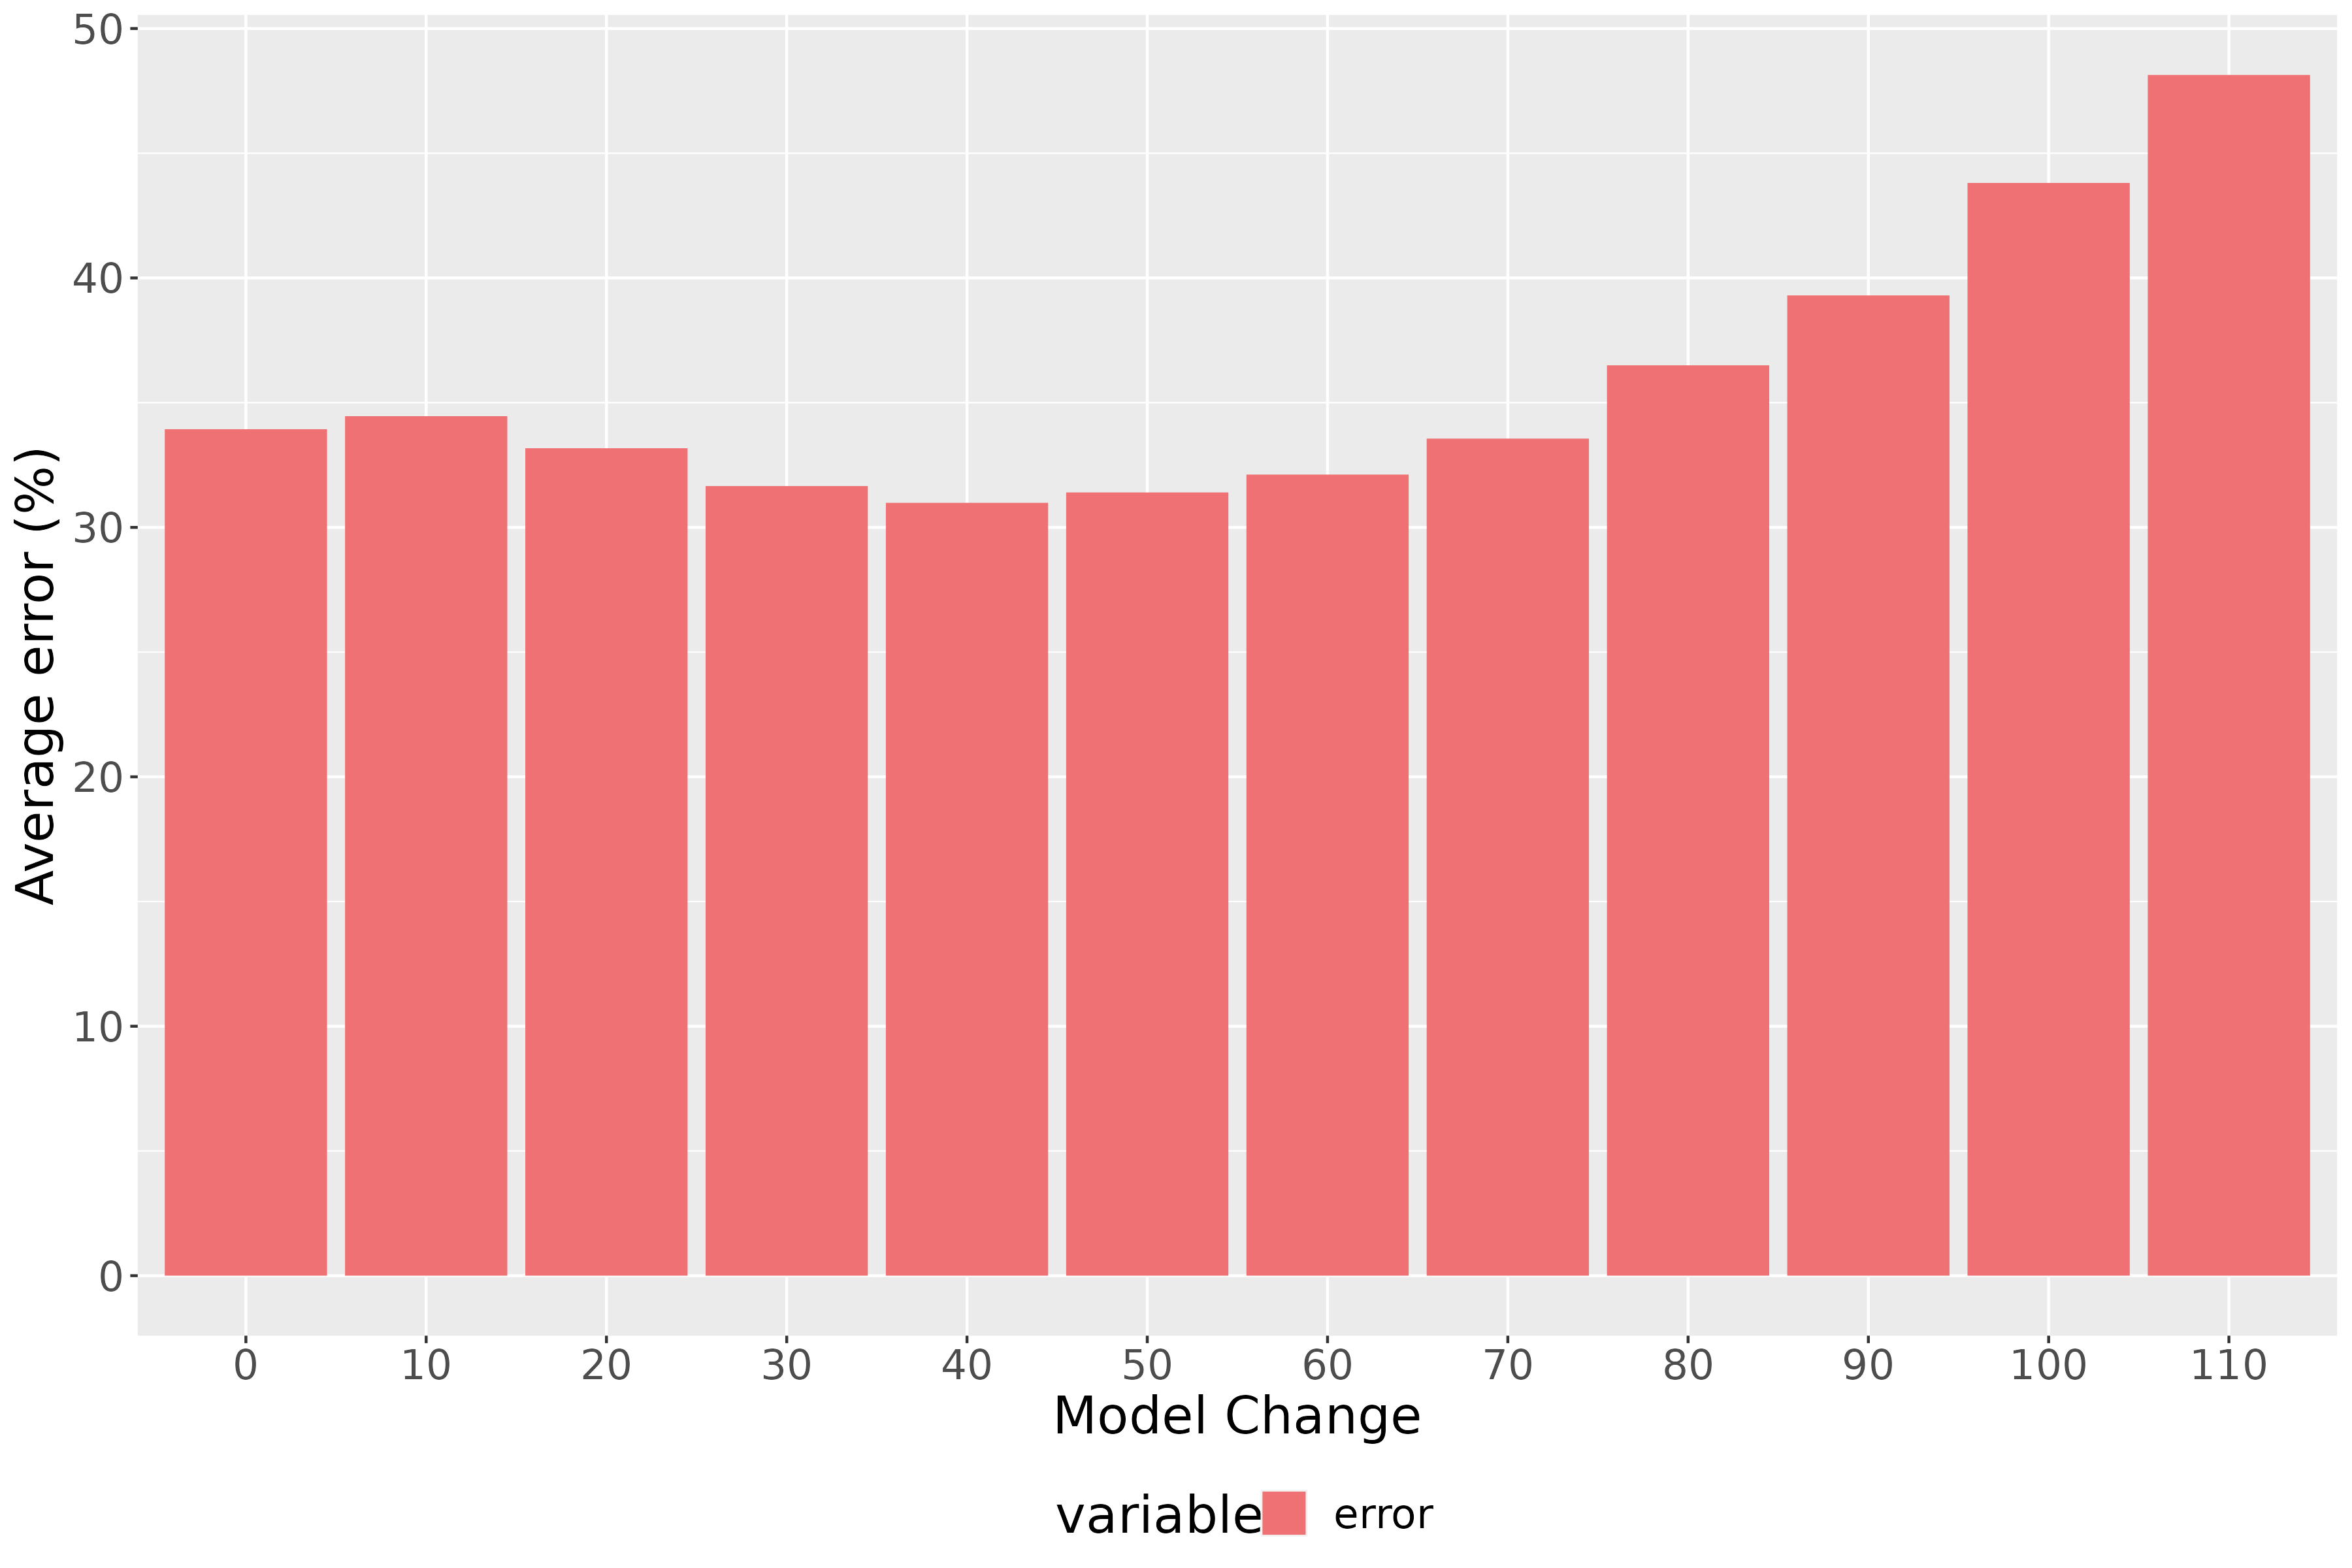
\includegraphics[width=0.8\textwidth]{6_model_change/OSU/modelChangeError_16nodes_1ppn_all.png}
    \caption{Average error across all OSU benchmarks, as a function of when we switch our network model (16 processes)}
    \label{fig:6_model_change:osu_16_error}
\end{figure}

\begin{figure}[!h]
    \centering
    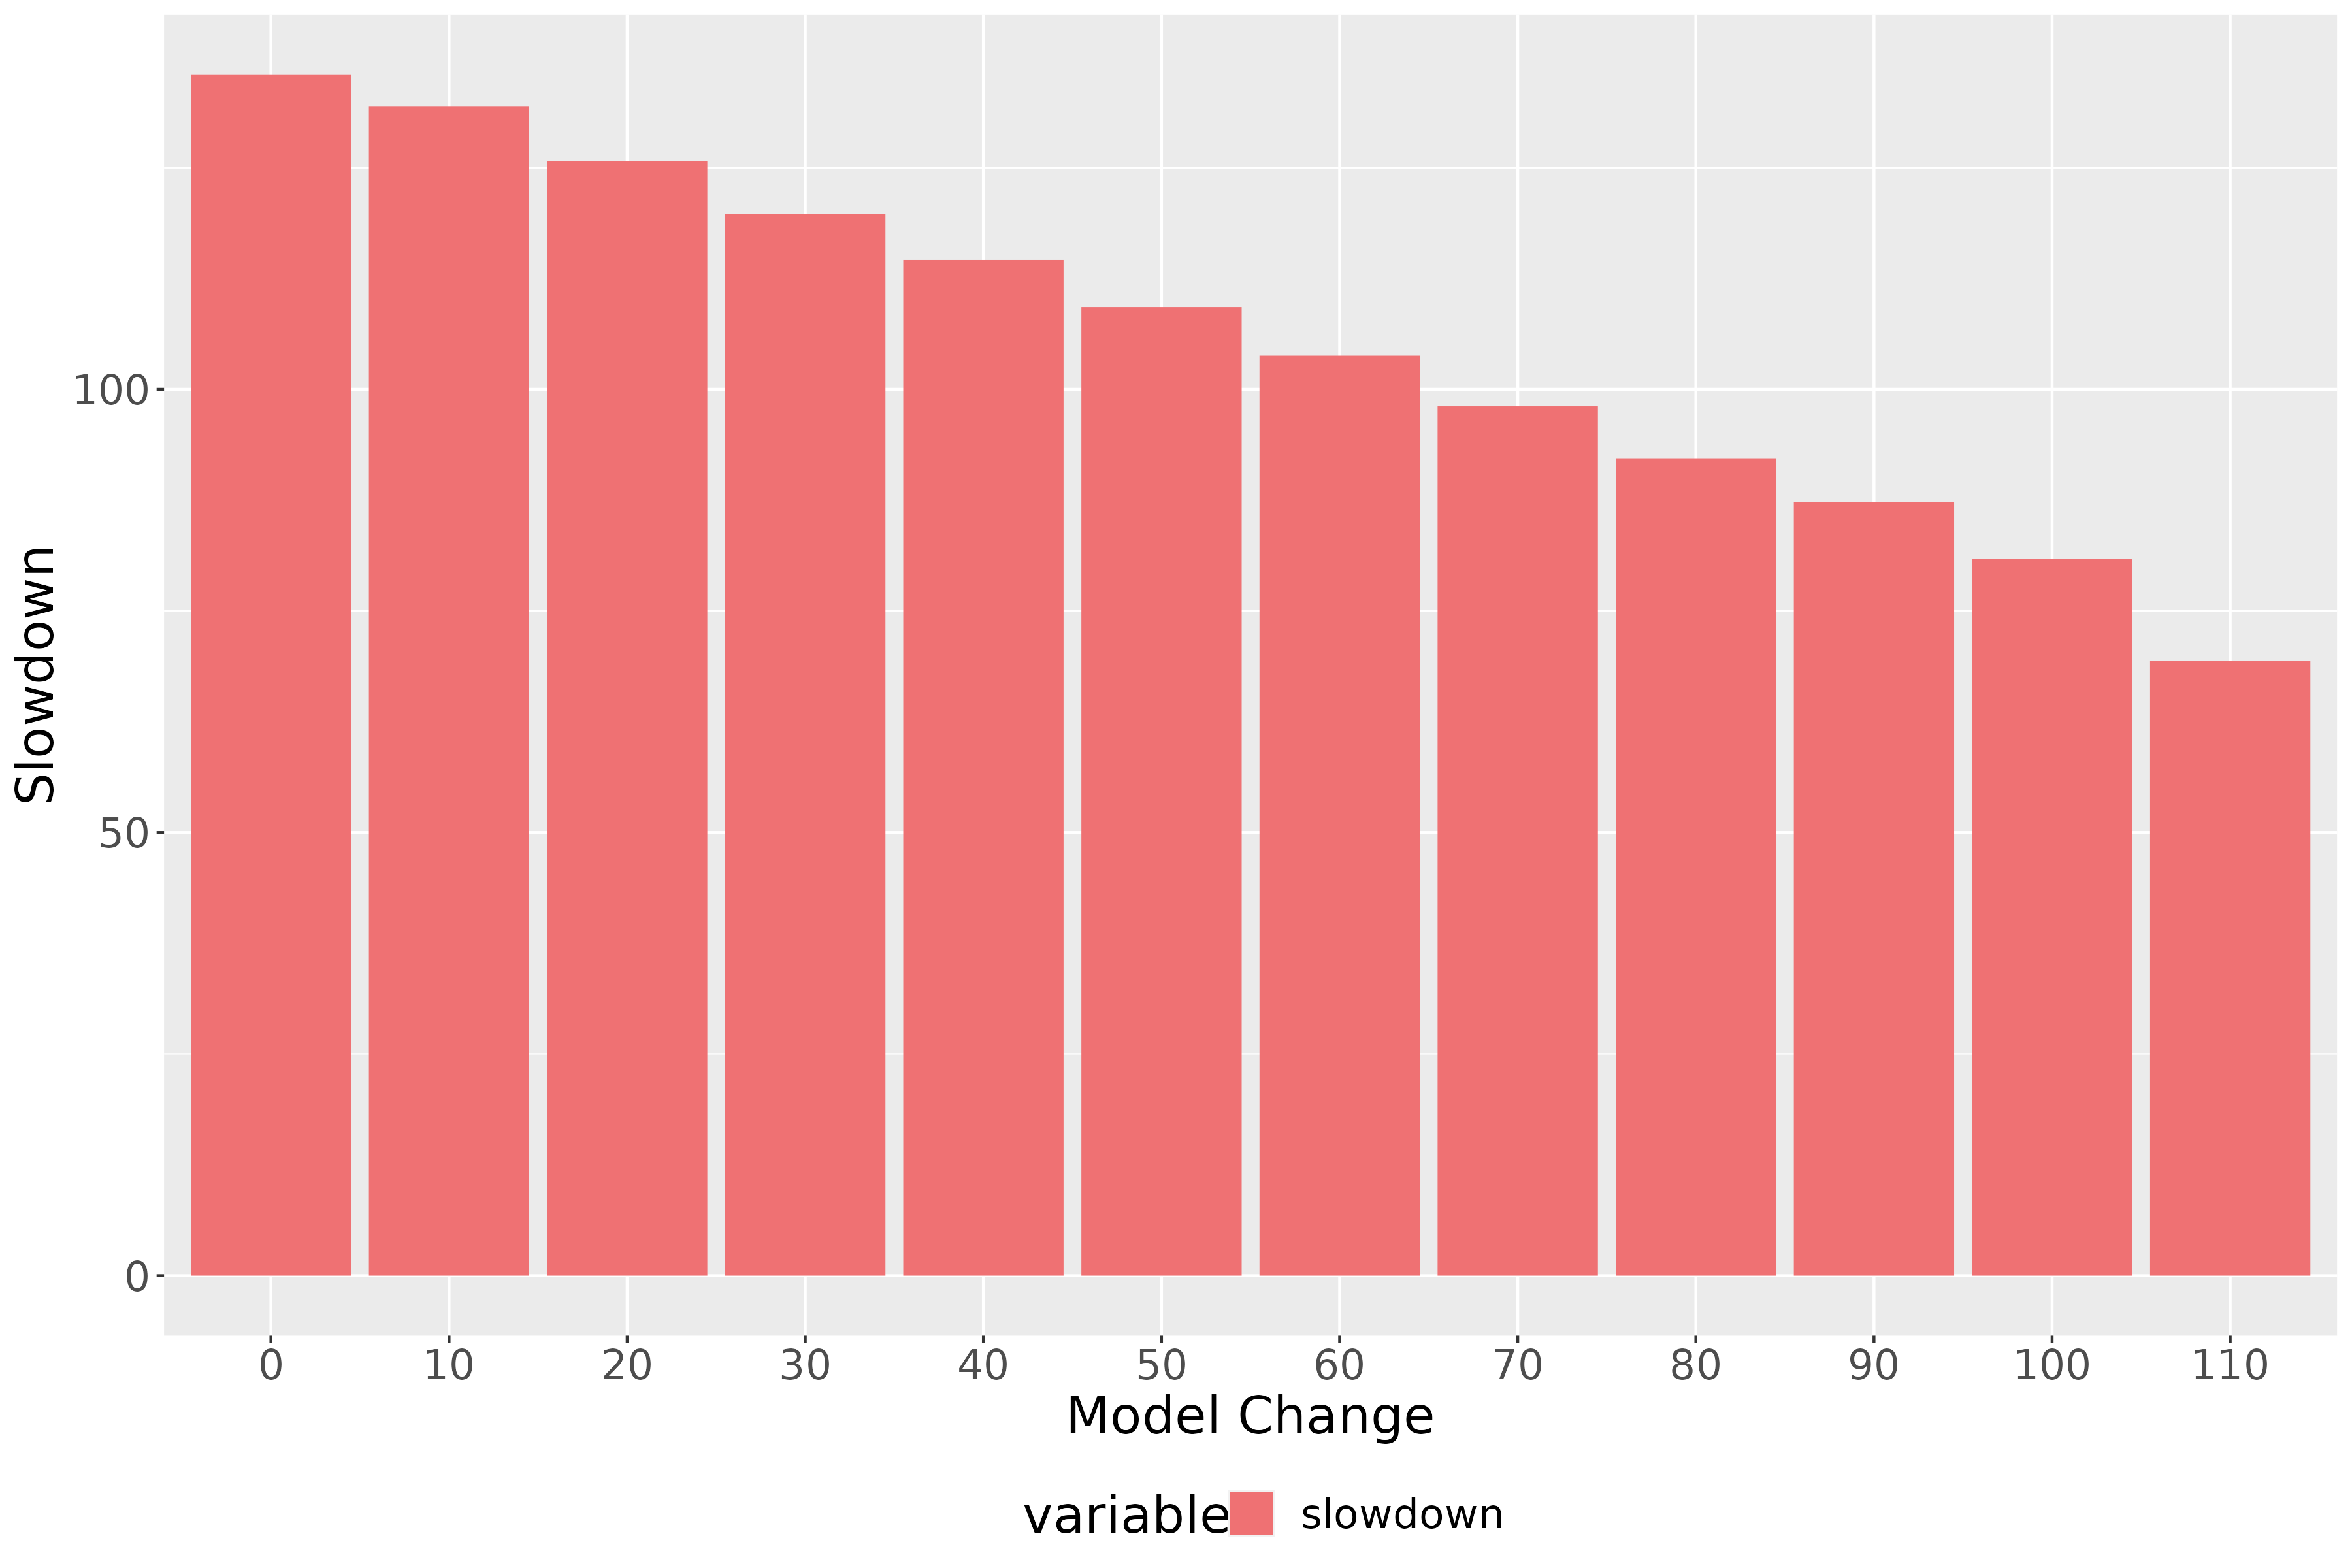
\includegraphics[width=0.8\textwidth]{6_model_change/OSU/modelChangeTime_16nodes_1ppn_all.png}
    \caption{Average slowdown across all OSU benchmarks, as a function of when we switch our network model (16 processes)}
    \label{fig:6_model_change:osu_16_perf}
\end{figure}

In order to change models in OSU micro-benchmarks, we set the number of
iterations over the benchmarked primitive to 110 (10 warmup ones and 100 measure
ones), using the benchmarks' configuration parameters. Then we added a check in
the code of each benchmark in order to switch model after a configurable number
of iterations. Each time we started with SMPI, and we switched to OpenMPI over
S4BXI after either 0 iterations (so instantly at startup), or 10, 20, 30, etc.
all the way to 110 (in which case OpenMPI over S4BXI is not used at all).
Plotting the results of our simulations is not trivial: there are 31 benchmarks,
11 different points at which we change models, and many message sizes. The
resulting data ends up spanning over four dimensions, therefore we had to make
choices about what to depict. We started by performing the same calculations
that we presented in Section~\ref{subsubsec:5_high_level:osu_results}, in which
we showed the average error and the slowdown of simulators. However, in this
section, we compare 11 different models (with a variable proportion of each
implementation) instead of just two, therefore it was not convenient to plot all
31 benchmarks side-by-side. For this reason, we will plot the average of the 31
average errors, and the average of the 31 slowdowns, as a function of when we
switch our network model.

From a technical point of view, we used similar settings as we did in
Chapter~\ref{chap:high_level}: executions on 16 nodes with one process per node,
as well as eight nodes with four processes per node, and simulations on one of
the machines from our real-world cluster.

For 16 MPI ranks, the accuracy of our simulation method is shown on
Figure~\ref{fig:6_model_change:osu_16_error}. As expected, an execution using
only OpenMPI over S4BXI (on the left) is more accurate than using only SMPI (on
the right). We can also see that there is little difference in accuracy if we
change models instantly or after ten iterations. This is also expected since the
first ten iterations are just warmup, and are not timed by the benchmark. In the
middle, we can see that, in this particular case,  the errors of both network
models cancel out for some benchmarks (in the case where one model is too
optimistic and the other too pessimistic), which gives us an even slightly lower
error than with only OpenMPI over S4BXI.

From a performance perspective, we can see on
Figure~\ref{fig:6_model_change:osu_16_perf} that the more we use SMPI, the
smaller the slowdown is, as expected.

\begin{figure}[!h]
    \centering
    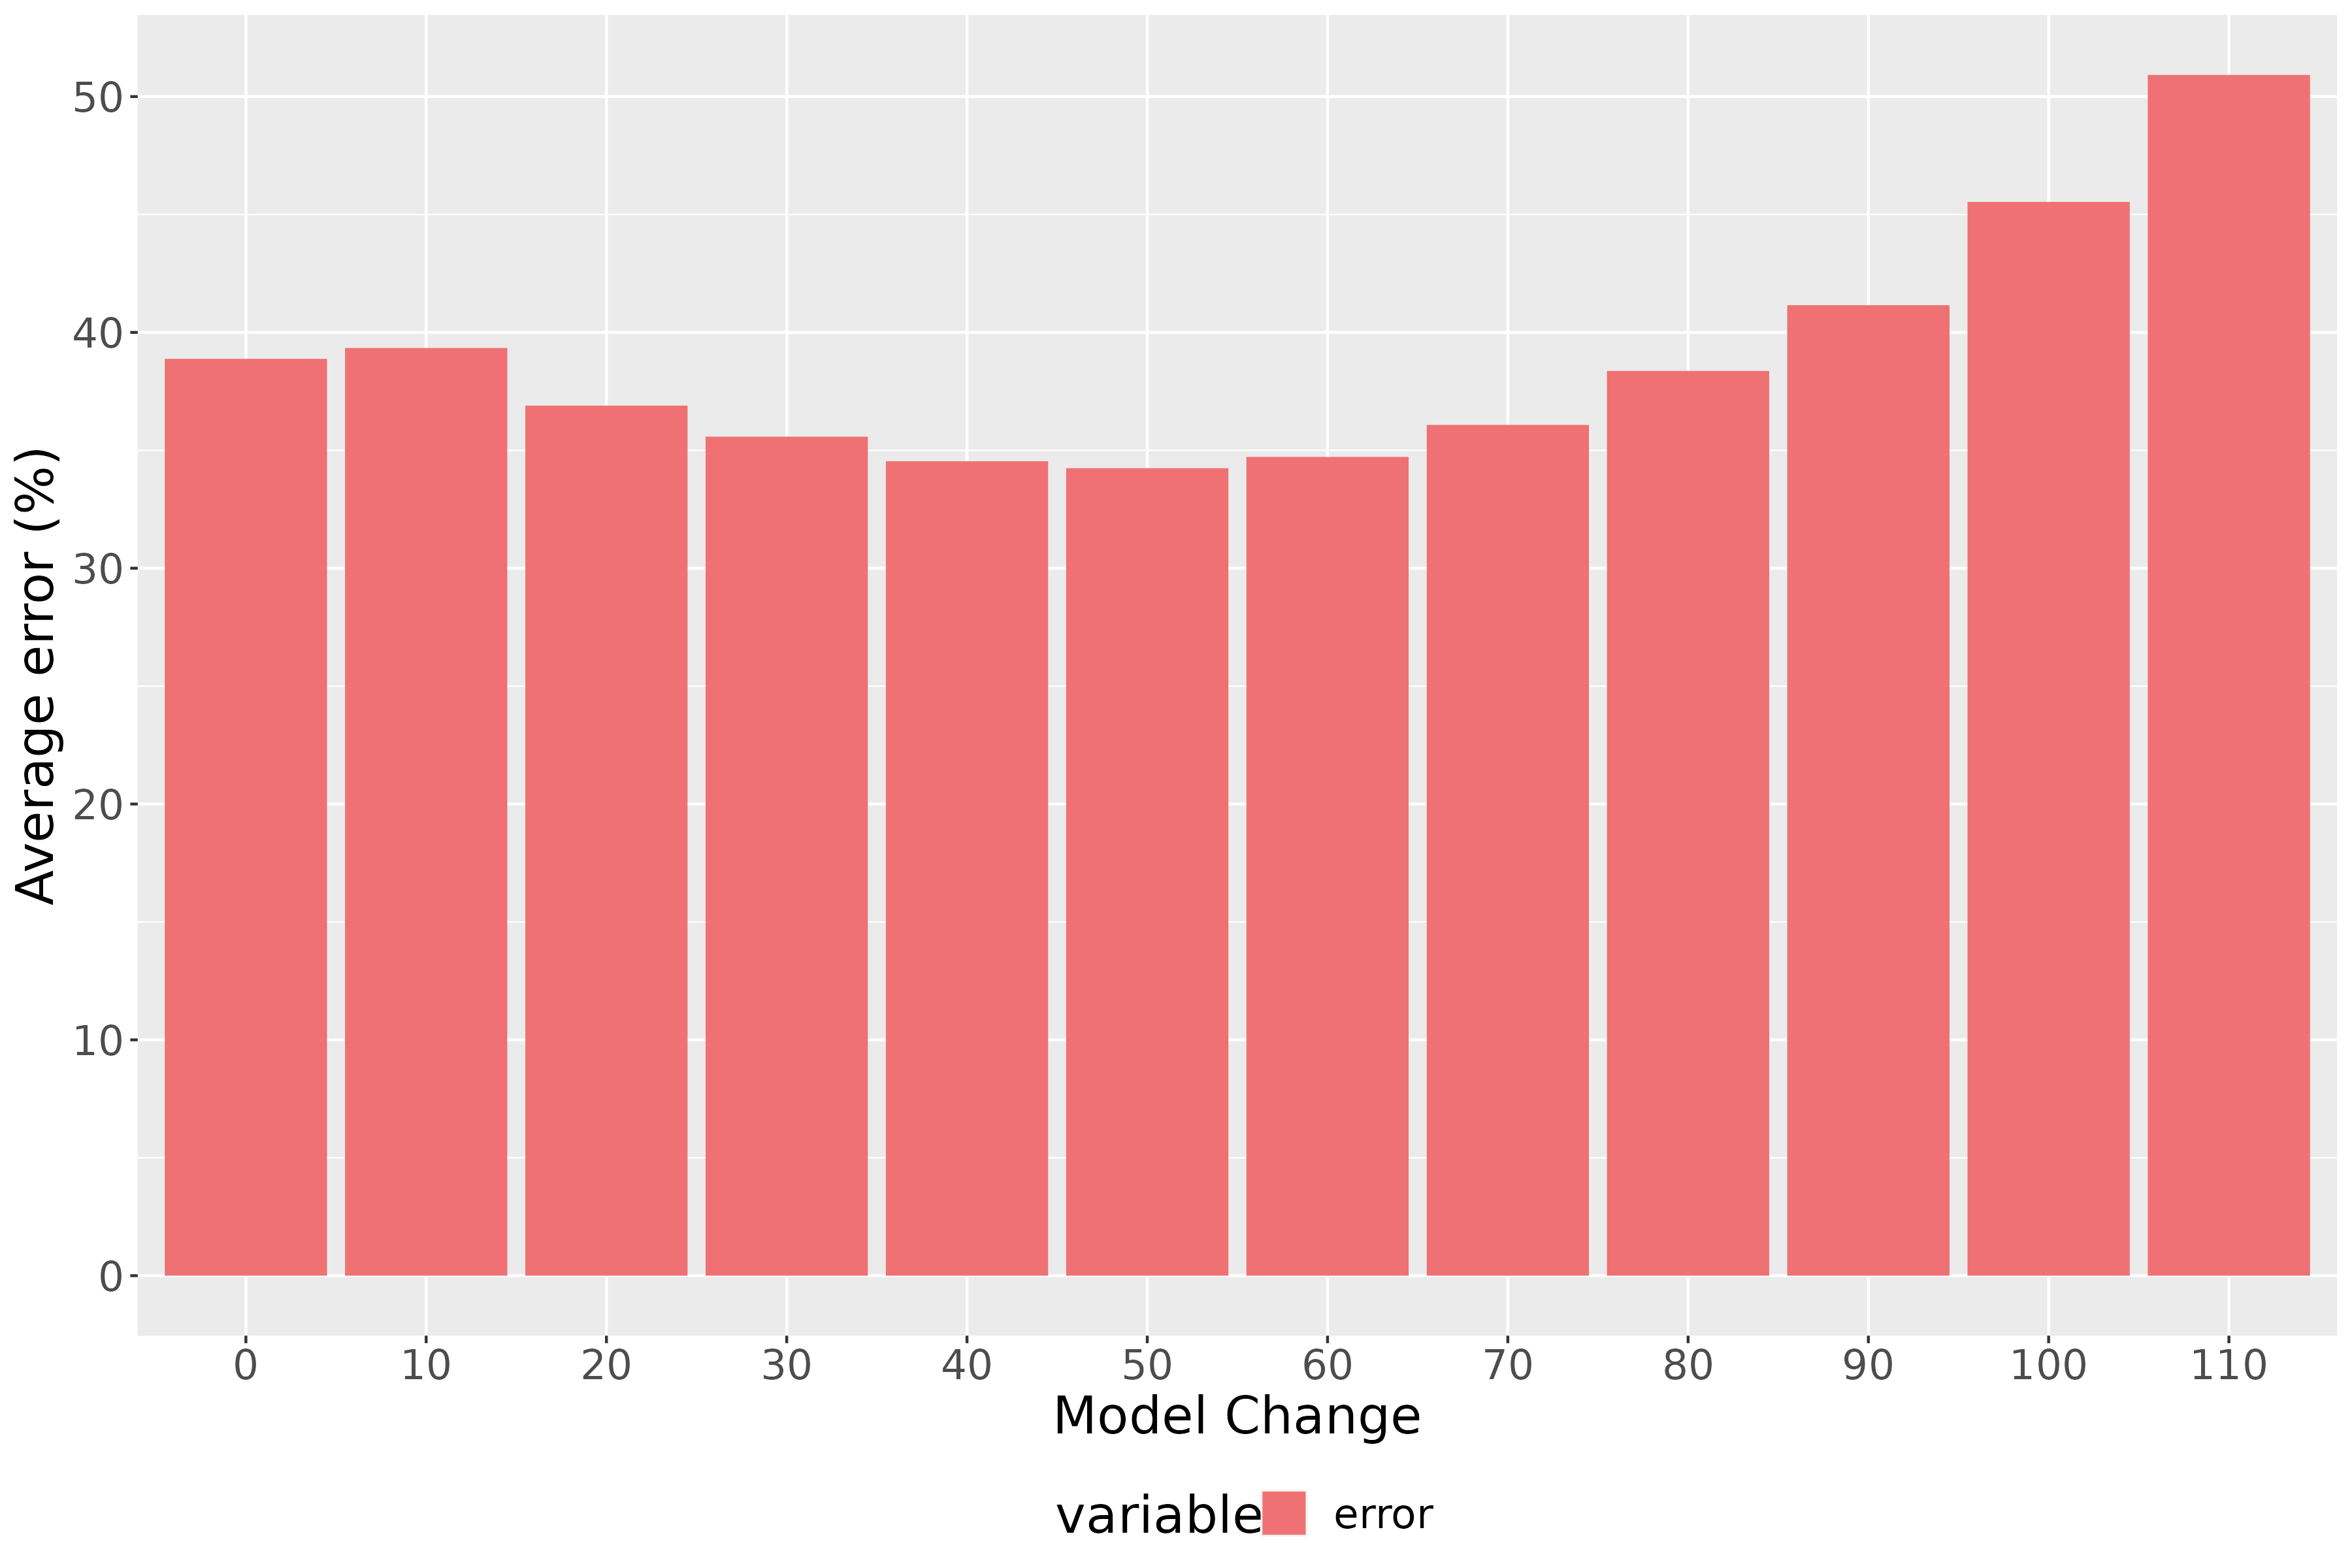
\includegraphics[width=0.8\textwidth]{6_model_change/OSU/modelChangeError_8nodes_4ppn_sync.png}
    \caption{Average error across synchronous OSU benchmarks, as a function of when we switch our network model (32 processes)}
    \label{fig:6_model_change:osu_32_sync_error}
\end{figure}

\begin{figure}[!h]
    \centering
    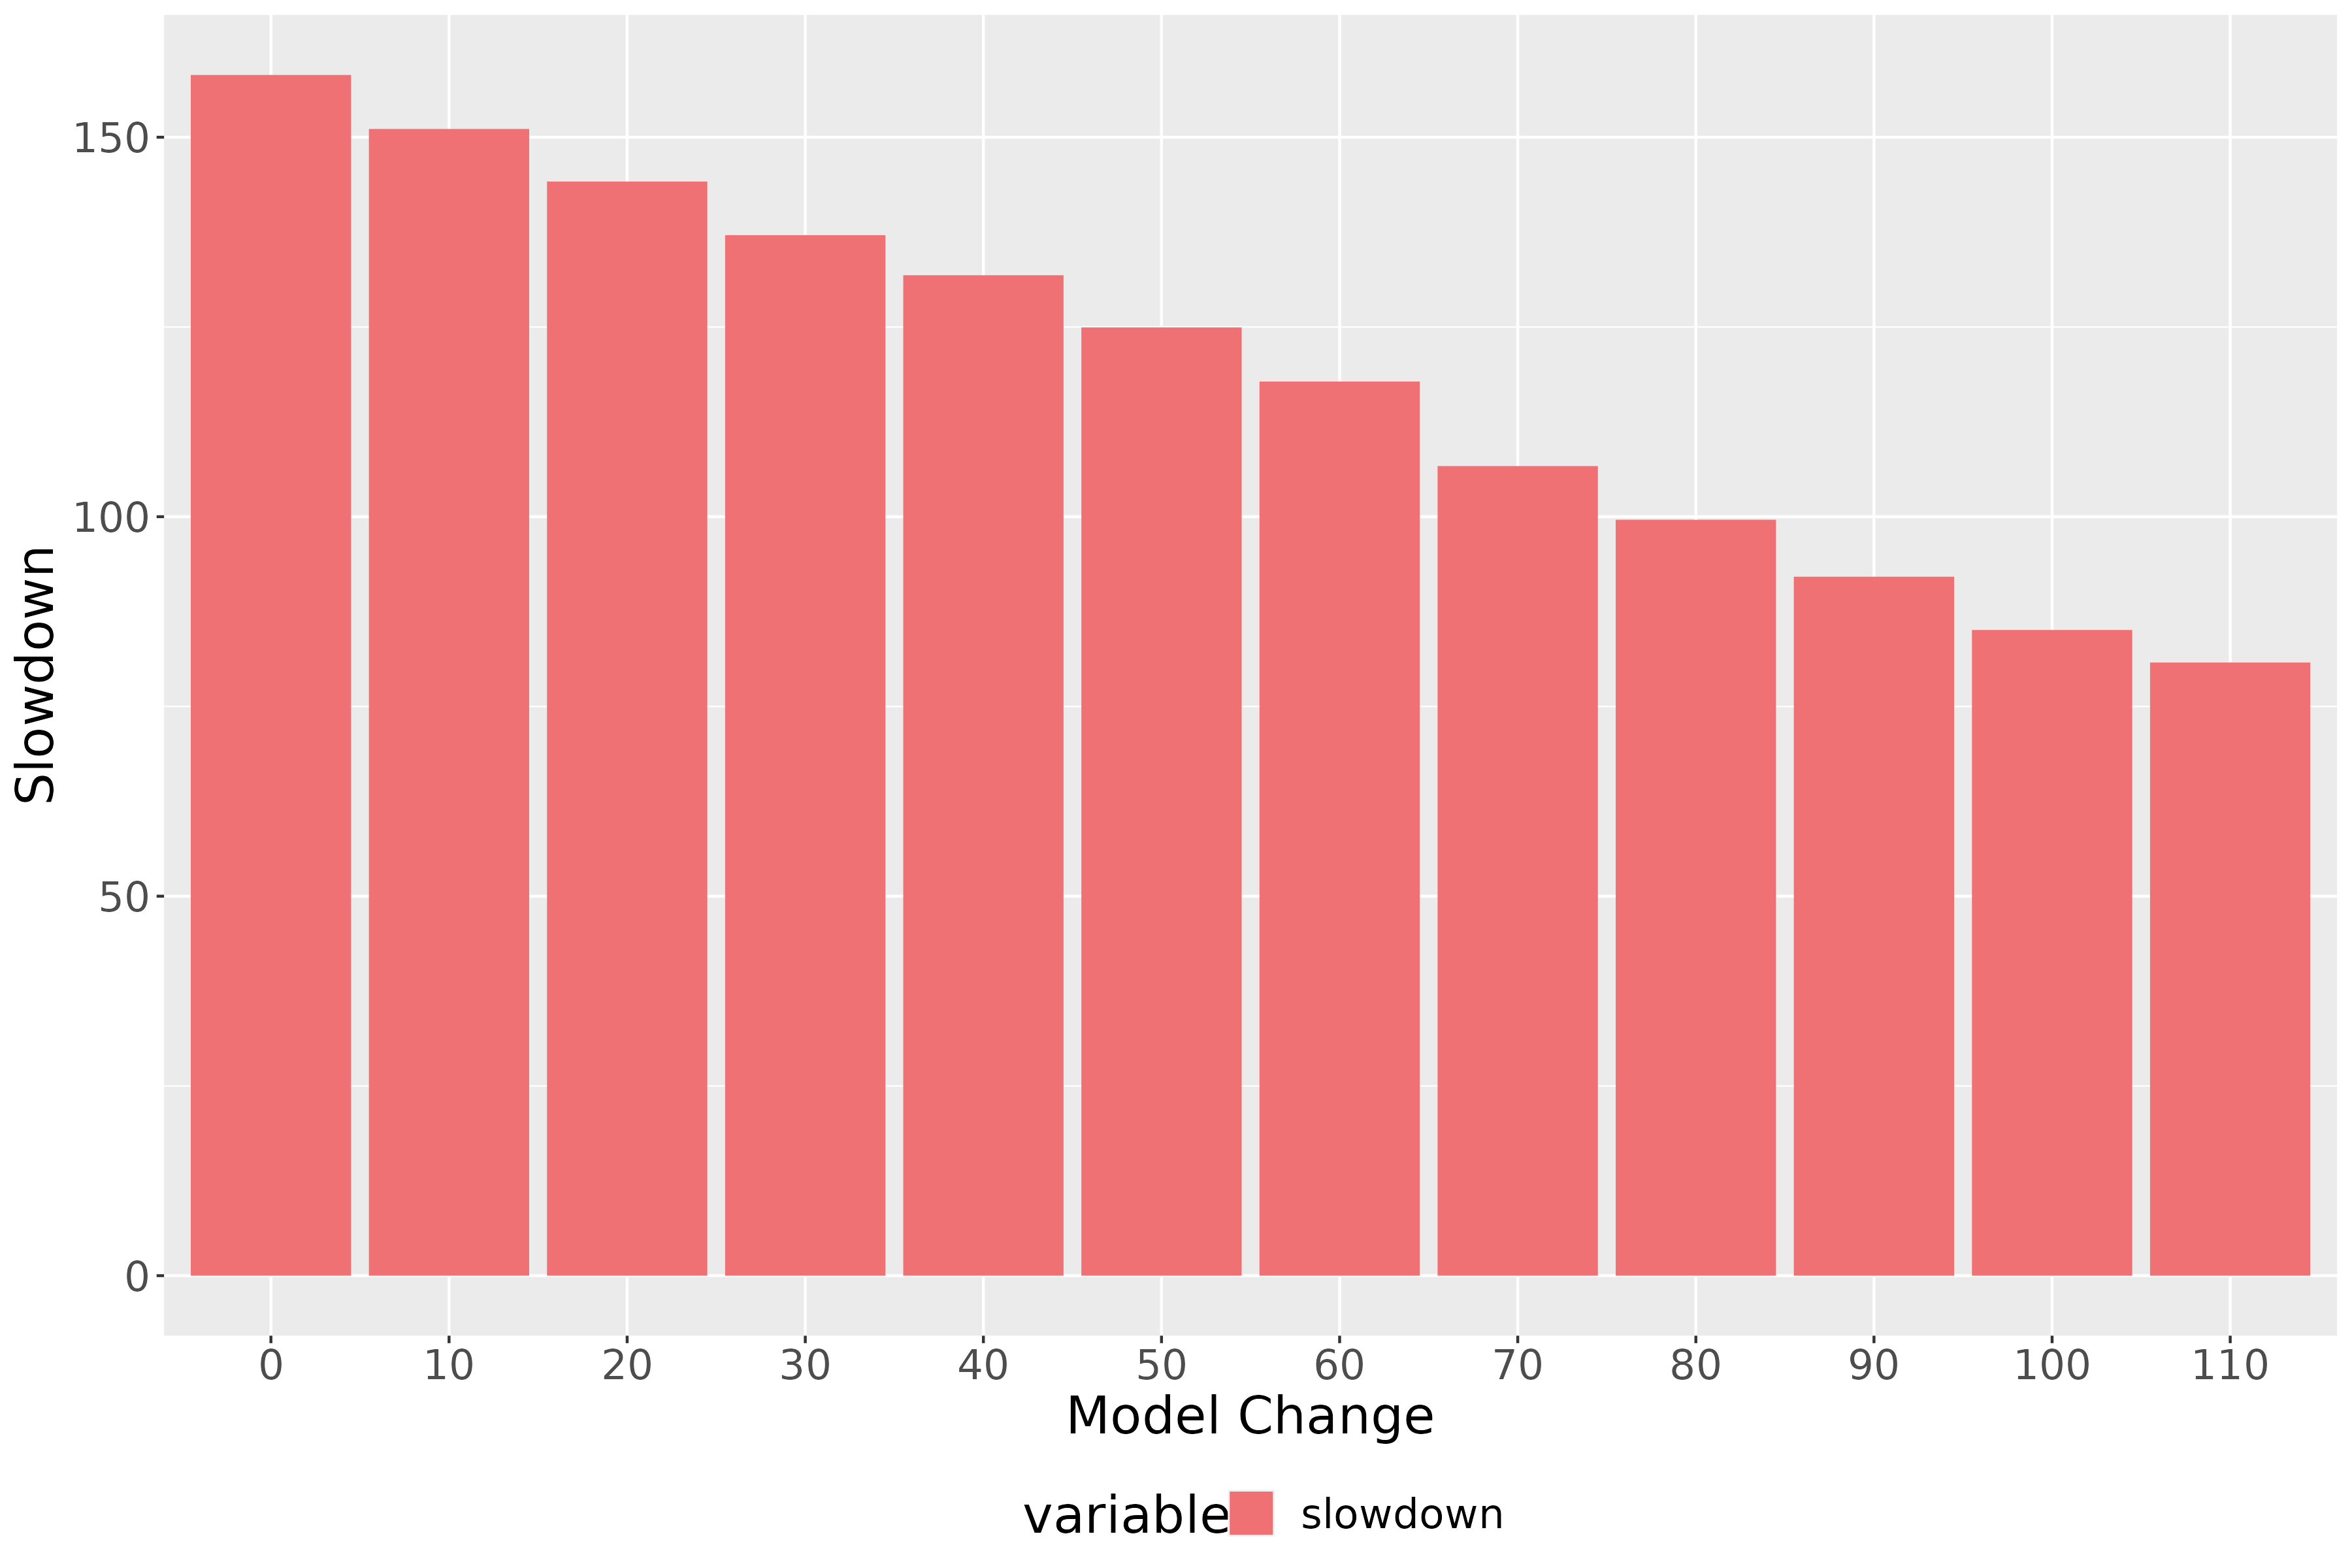
\includegraphics[width=0.8\textwidth]{6_model_change/OSU/modelChangeTime_8nodes_4ppn_sync.png}
    \caption{Average slowdown across synchronous OSU benchmarks, as a function of when we switch our network model (32 processes)}
    \label{fig:6_model_change:osu_32_sync_perf}
\end{figure}

For 32 MPI ranks on the other hand (8 nodes and 4 processes per node), the
results are a bit different. We need to differentiate two cases, which give us
very different results: synchronous and asynchronous operations. In the case of
synchronous operations, we get the similar results as with 16 MPI ranks, as
depicted in Figure~\ref{fig:6_model_change:osu_32_sync_error} for the accuracy,
and Figure~\ref{fig:6_model_change:osu_32_sync_perf} for the performance of our
simulations.

\begin{figure}[!h]
    \centering
    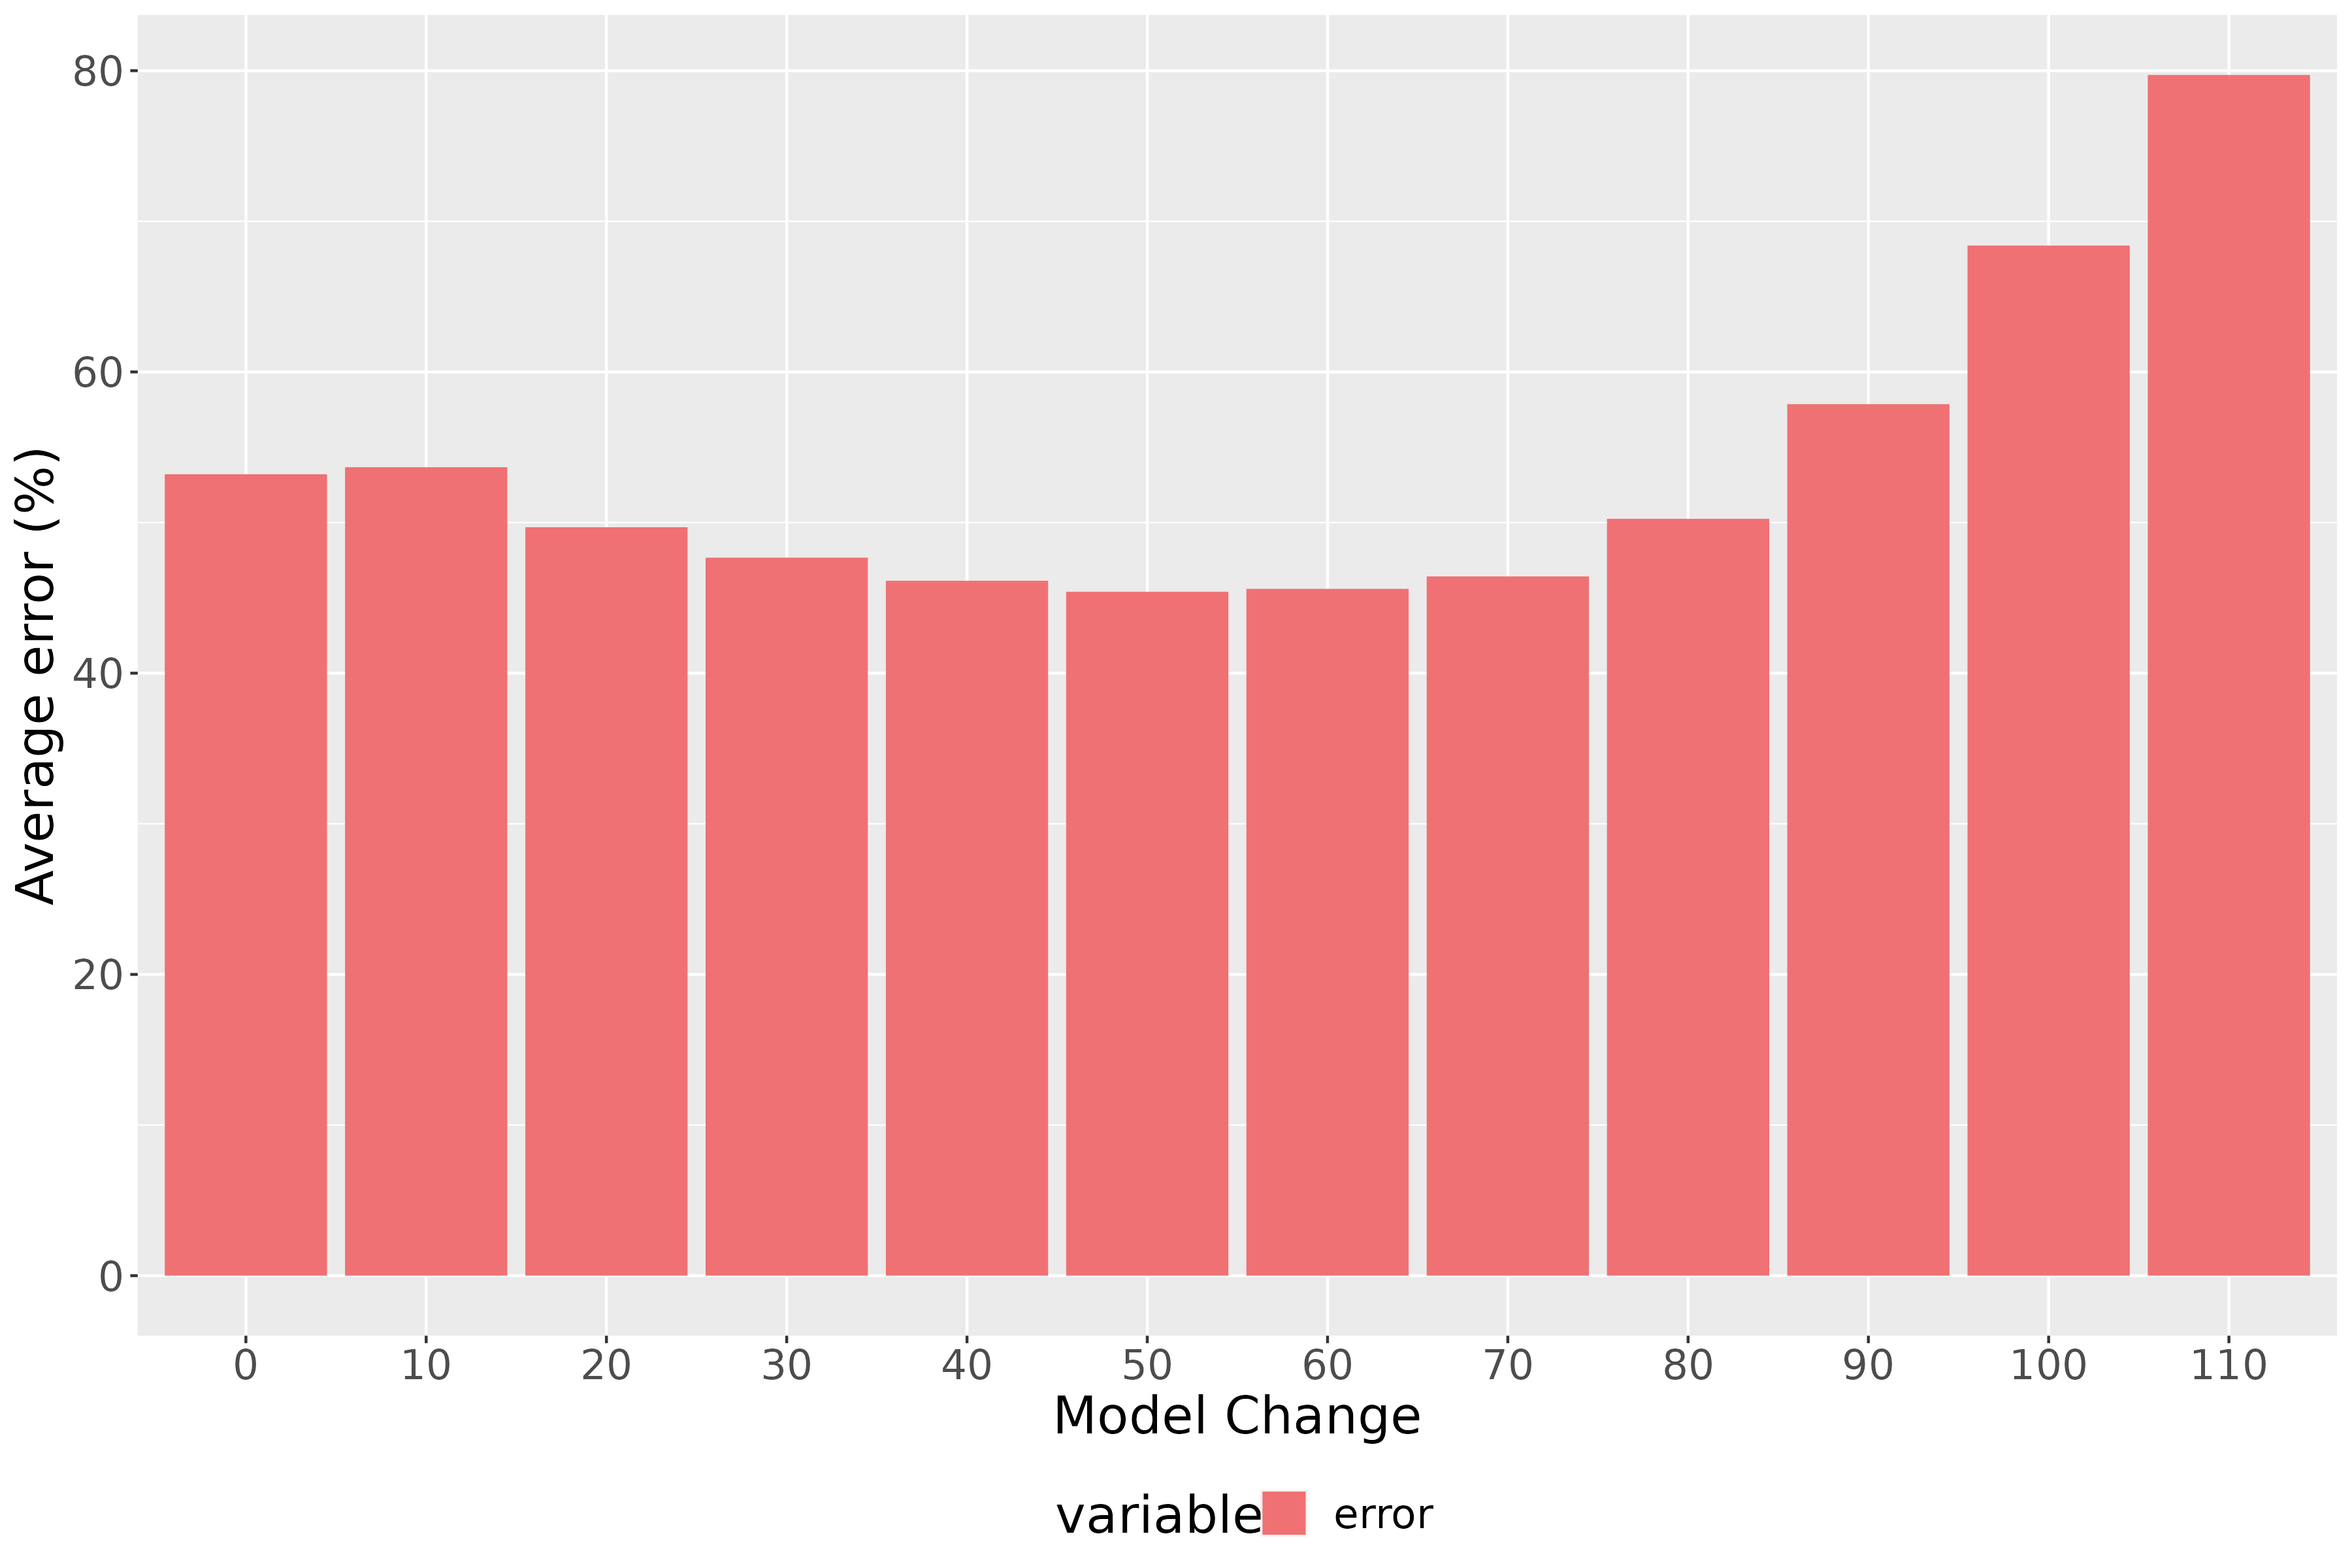
\includegraphics[width=0.8\textwidth]{6_model_change/OSU/modelChangeError_8nodes_4ppn_async.png}
    \caption{Average error across asynchronous OSU benchmarks, as a function of when we switch our network model (32 processes)}
    \label{fig:6_model_change:osu_32_async_error}
\end{figure}

\begin{figure}[!h]
    \centering
    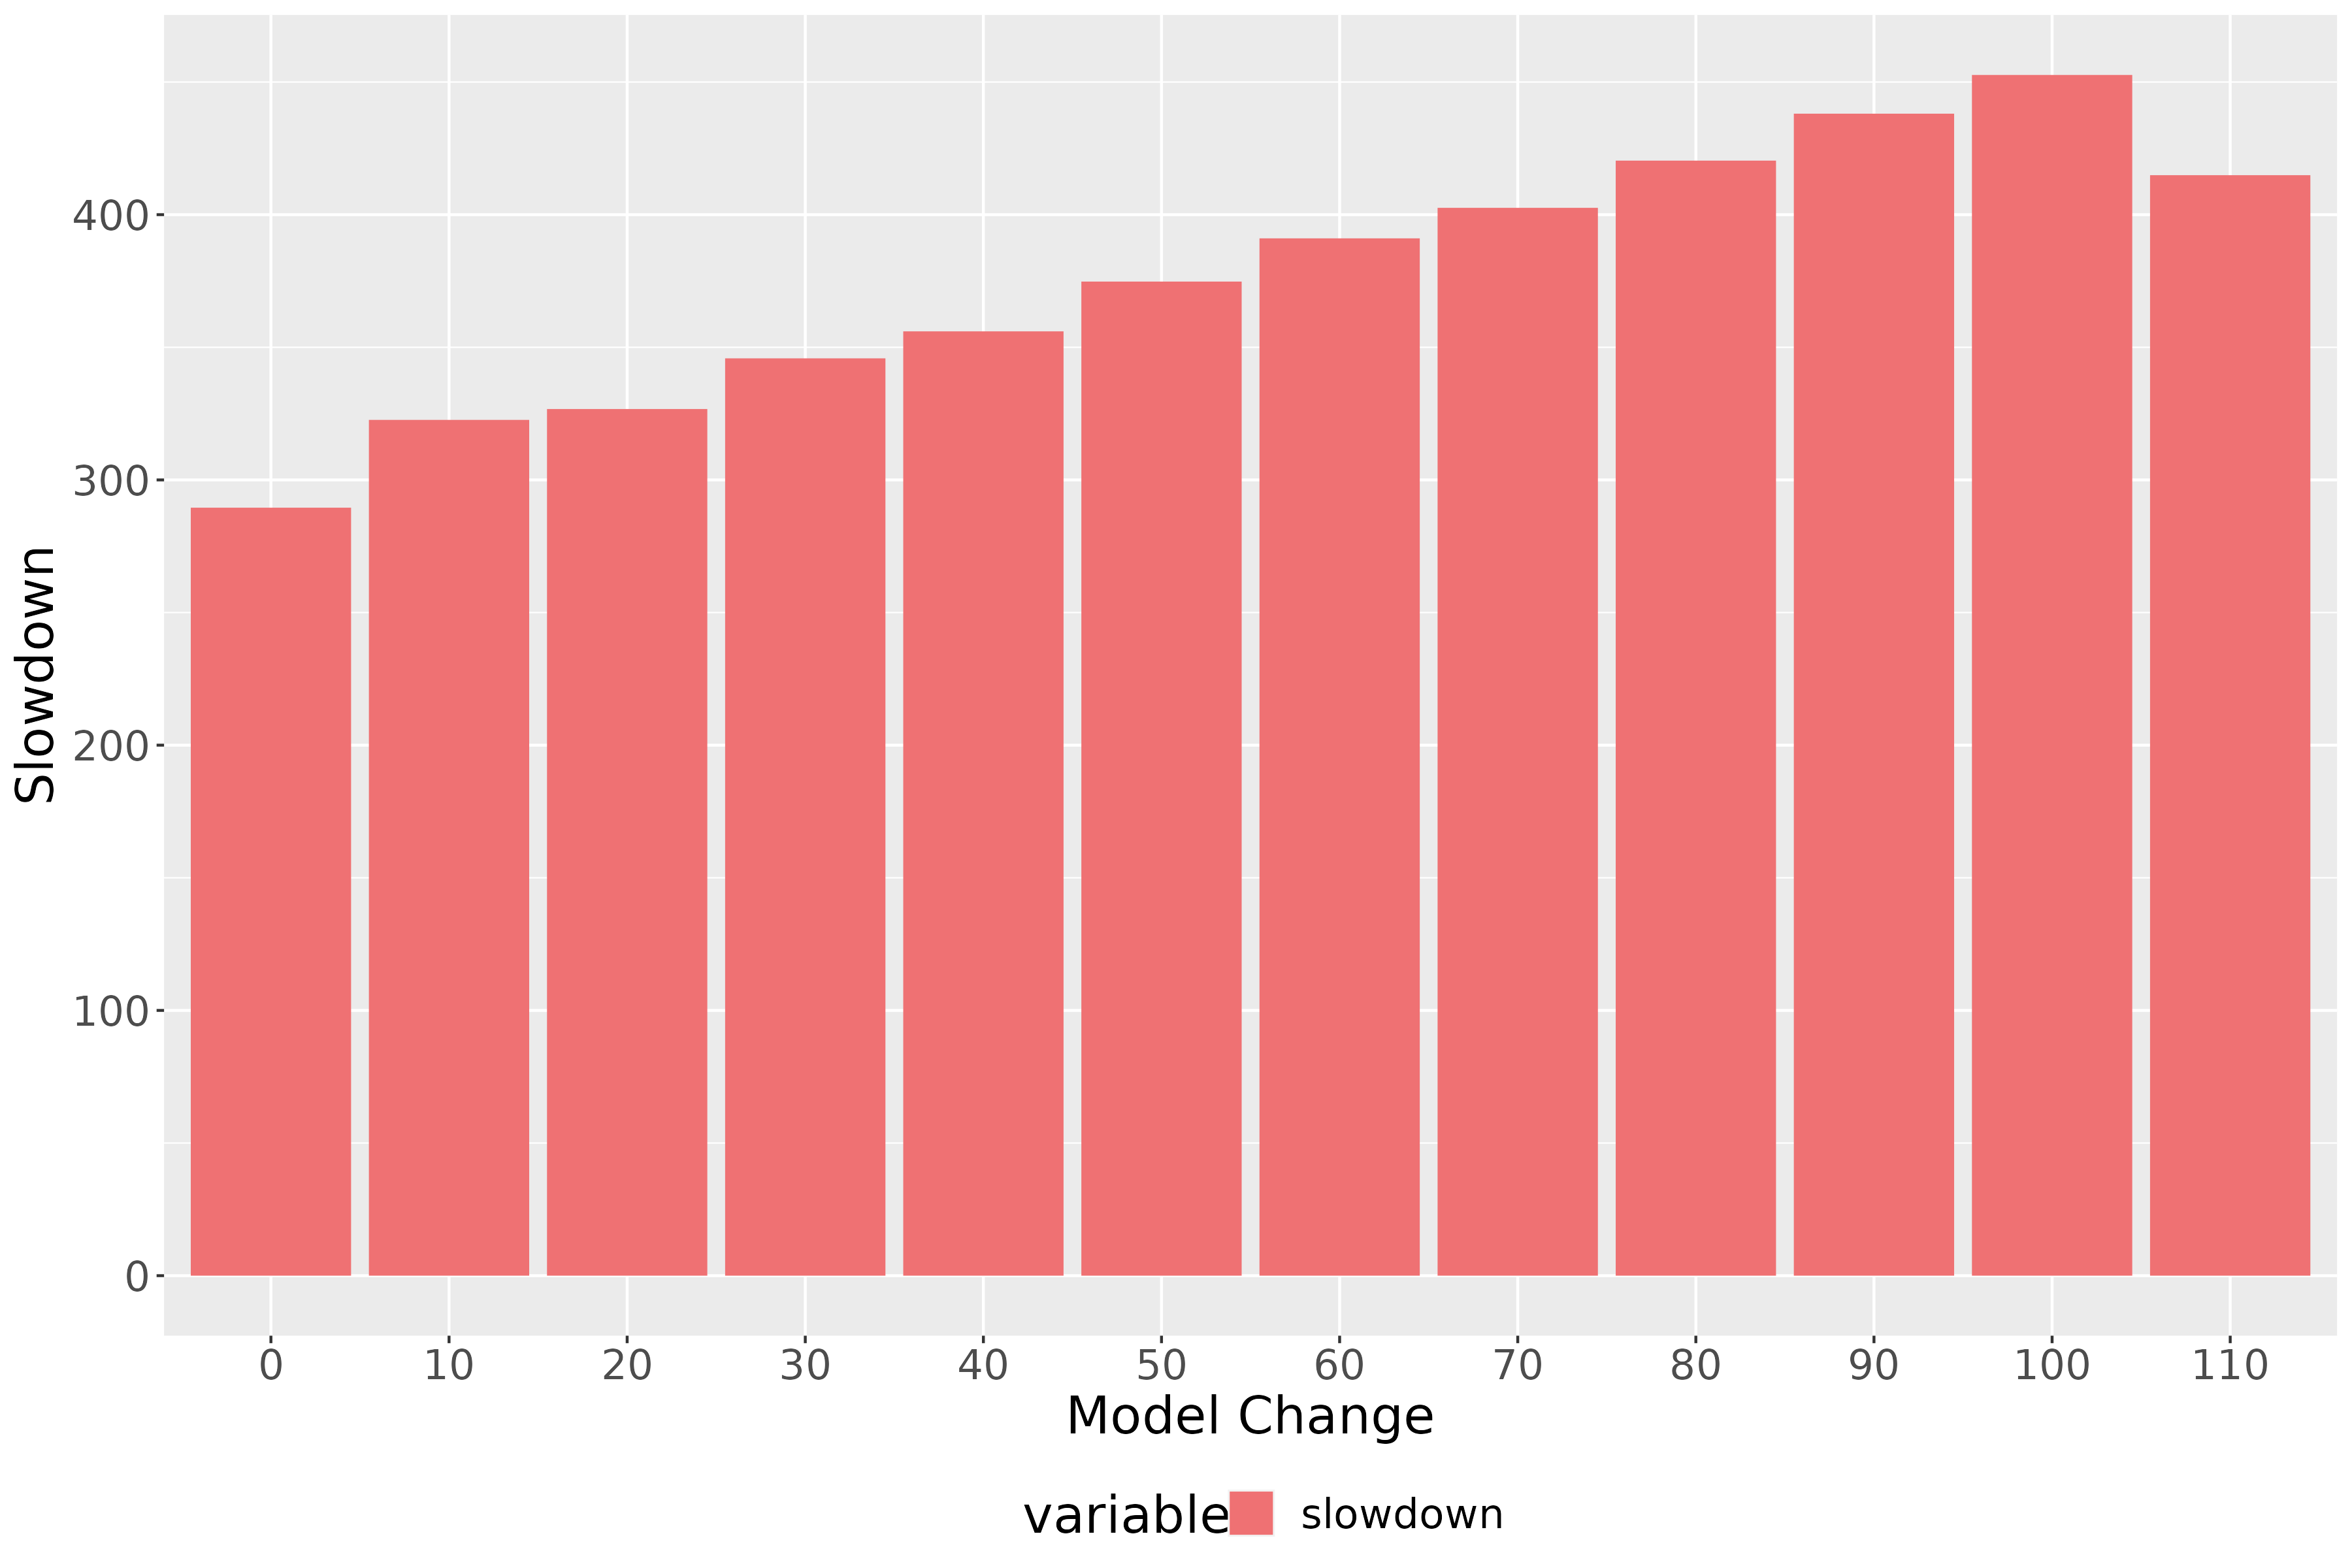
\includegraphics[width=0.8\textwidth]{6_model_change/OSU/modelChangeTime_8nodes_4ppn_async.png}
    \caption{Average slowdown across asynchronous OSU benchmarks, as a function of when we switch our network model (32 processes)}
    \label{fig:6_model_change:osu_32_async_perf}
\end{figure}

For asynchronous operations, the results are way more variable between the
different operations (in particular the IAllGather primitive is very pathologic
in SMPI), and therefore looking at averages is not as meaningful. For accuracy,
we can see on Figure~\ref{fig:6_model_change:osu_32_async_error} that the
results are similar to everything we have seen so far: our approach performs
better than SMPI in average, and if we change models around the middle of each
benchmark we get an even better accuracy because errors from both models cancel
out (luckily). From a performance perspective on the other hand,
Figure~\ref{fig:6_model_change:osu_32_async_perf} shows that our approach is
faster than SMPI, even though our model is more detailed. This is unexpected,
but after discussing asynchronous collectives with SimGrid's development team,
it seems that these operations are rarely used in real applications (indeed, we
never encountered them in our studies), and therefore there has been less work
put into optimizing them. This is why we did not spend more time studying them
in more detail. Instead, we decided to benchmark more realistic applications.

\subsection{Quicksilver}

After testing our approach for model changes on OSU benchmarks, we tried it on
Quicksilver: since this application performs ten cycles of computation, that are
relatively independent, it was easy to add model changes between cycles in the
code. Therefore, we executed Quicksilver in simulation for 11 different
configurations: we always started with SMPI, and then we switched to our
approach after a variable number of cycles. As a result, we have eleven
simulations for 100\% SMPI usage, 90\% SMPI usage, 80\%, etc. all the way to
0\%, if we switch to OpenMPI over S4BXI immediately at startup. From a technical
perspective, simulations are executed on a desktop computer, which has an Intel®
Core™ i9-10850K CPU and 32 GB of RAM. Once again, the resulting data is very
large, as these model changes add a new variable to our simulations, along with
the existing ones: number of nodes used, number of processes per node and number
of initial particles fed to Quicksilver (which correspond to the problem size).
As a result, we will not study every graph, but instead we will explain the
trends that we observed when each variable changes.

\begin{figure}[!ht]
    \centering
    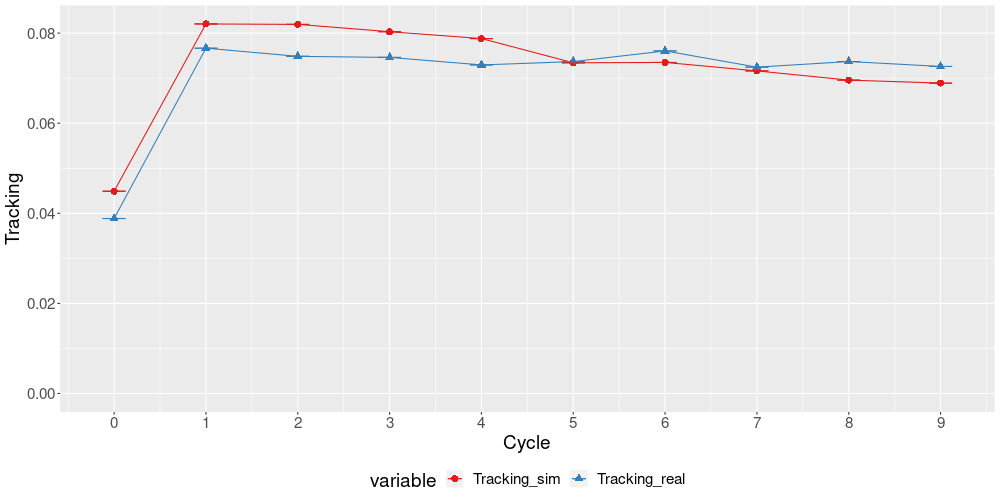
\includegraphics[width=\textwidth]{6_model_change/Quicksilver/s4bxi_10000particles_modelChange5_4tasks_1ppn.png}
    \caption{Accuracy of Quicksilver's simulation on 4 MPI ranks, with a model change from SMPI to our approach after cycle n°4, with 10,000 input particles}
    \label{fig:6_model_change:quicksilver_4tasks_1ppn_accuracy}
\end{figure}

\begin{figure}[!ht]
    \centering
    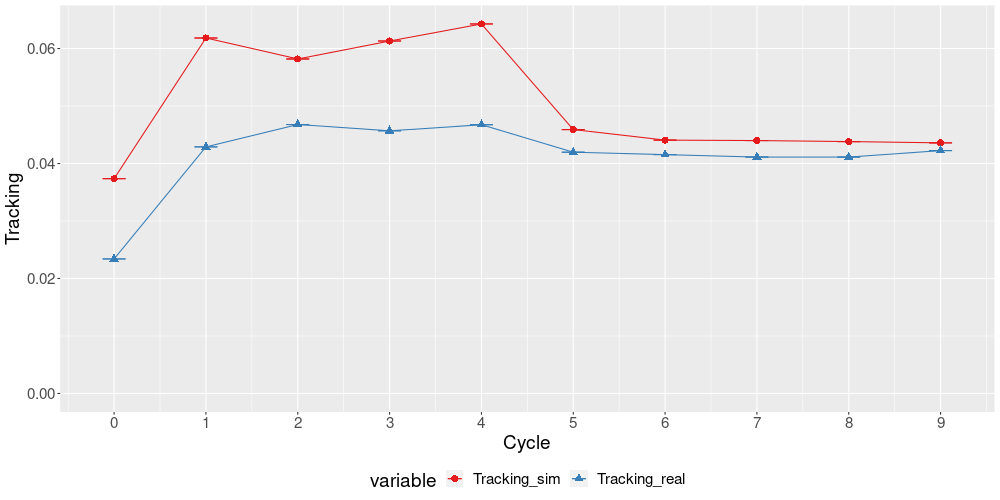
\includegraphics[width=\textwidth]{6_model_change/Quicksilver/s4bxi_10000particles_modelChange5_8tasks_1ppn.png}
    \caption{Accuracy of Quicksilver's simulation on 8 MPI ranks, with a model change from SMPI to our approach after cycle n°4, with 10,000 input particles}
    \label{fig:6_model_change:quicksilver_8tasks_1ppn_accuracy}
\end{figure}

\begin{figure}[!ht]
    \centering
    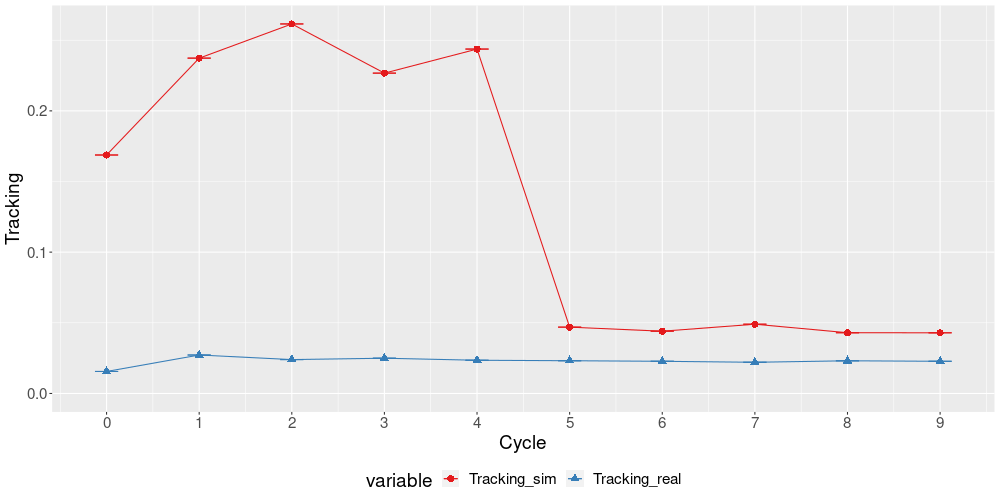
\includegraphics[width=\textwidth]{6_model_change/Quicksilver/s4bxi_10000particles_modelChange5_16tasks_1ppn.png}
    \caption{Accuracy of Quicksilver's simulation on 16 MPI ranks, with a model change from SMPI to our approach after cycle n°4, with 10,000 input particles}
    \label{fig:6_model_change:quicksilver_16tasks_1ppn_accuracy}
\end{figure}

Regarding accuracy, the simulations behave as we expect based on the results of
Chapter~\ref{chap:high_level}: as we have seen in
Section~\ref{subsec:5_high_level:quicksilver}, SMPI shows a good accuracy as
long as we model a small number of MPI ranks. To visualize this, we plotted the
result of three different simulations: all of them use 10,000 input particles,
and they switch from SMPI to OpenMPI between the iterations four and five,
therefore the left part of each figure shows SMPI's accuracy, and the right part
shows our approach's accuracy.
Figure~\ref{fig:6_model_change:quicksilver_4tasks_1ppn_accuracy} shows that the
accuracy remains good during the whole simulation if we run Quicksilver on four
MPI ranks (four nodes and one process per node). On the other hand,
Figure~\ref{fig:6_model_change:quicksilver_8tasks_1ppn_accuracy} shows a lack of
accuracy at the start of the simulation when we use eight MPI ranks (eight nodes
and one process per node). Finally,
Figure~\ref{fig:6_model_change:quicksilver_16tasks_1ppn_accuracy} shows that
this lack of accuracy of the SMPI part of the simulation only increases with the
number of MPI ranks, as we have seen previously, since the figure depicts a run
on 16 MPI ranks (16 nodes and one process per node). In all cases, when we
switch to the OpenMPI model, the accuracy improves, as expected.

\begin{figure}[!ht]
    \centering
    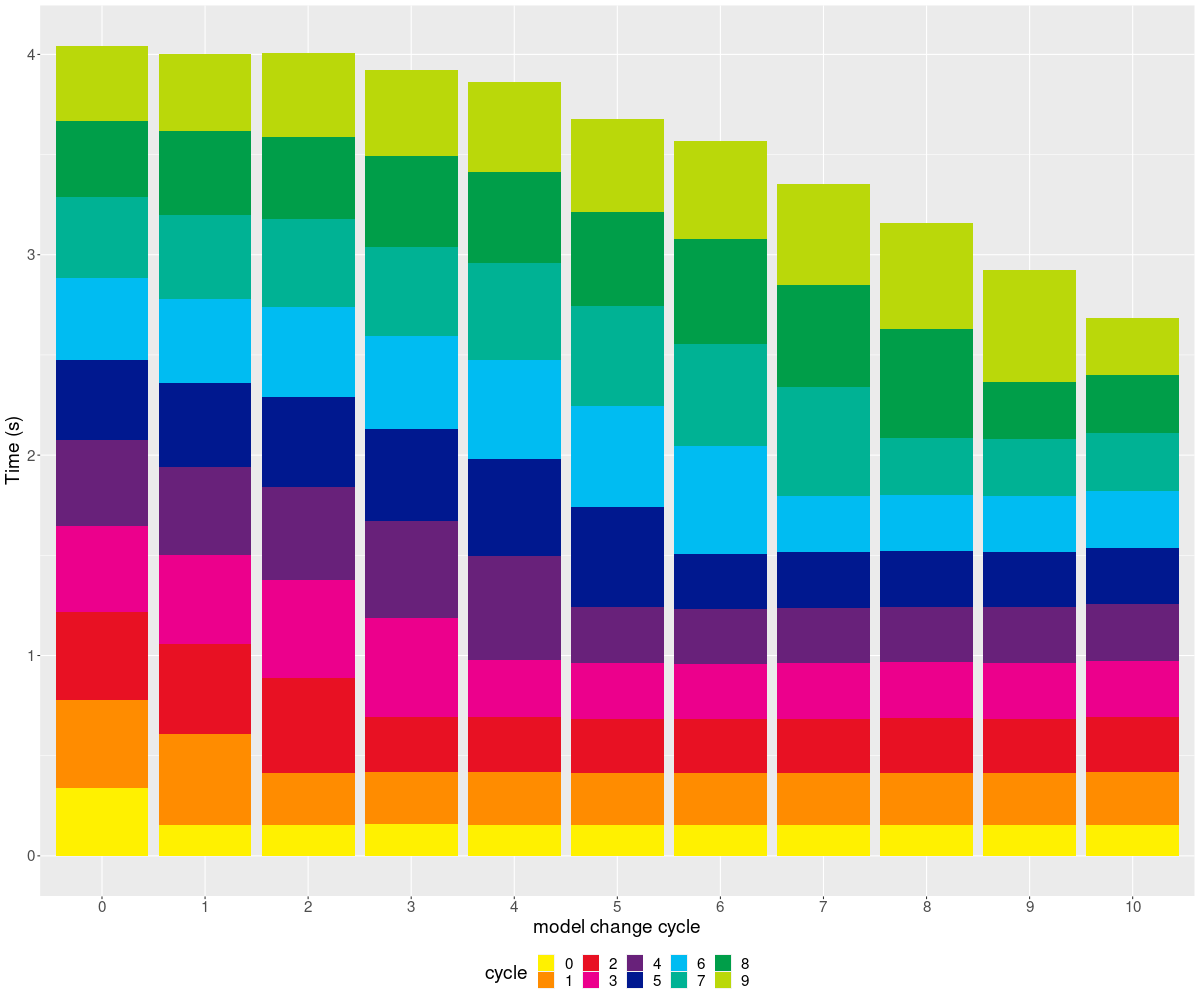
\includegraphics[width=\textwidth]{6_model_change/Quicksilver/cycle_log_wallclock_10000particles_4tasks_1ppn.png}
    \caption{Performance of Quicksilver's simulation on 4 MPI ranks, with 10,000 input particles}
    \label{fig:6_model_change:quicksilver_4tasks_1ppn_perf}
\end{figure}

From a performance perspective, the results that we obtain are more surprising.
In an attempt to better understand our data, we plot the performance of the
simulation for each model change position, therefore we have 11 bars that each
represent a simulation. However, inside each bar, we also display the
performance of each cycle individually, with the first cycle at the bottom, and
the last one at the top.
Figure~\ref{fig:6_model_change:quicksilver_4tasks_1ppn_perf} shows the
performance of simulations on four MPI ranks, and we can see that our model
changes behave as expected: the simulation using only our approach (highest bar
on the left) is slower than a fully SMPI simulation (lowest bar on the right),
and in between the performance improves (lower and lower bars) as we increase
the proportion of SMPI use.

\begin{figure}[!p]
    \centering\vspace{-3ex}
    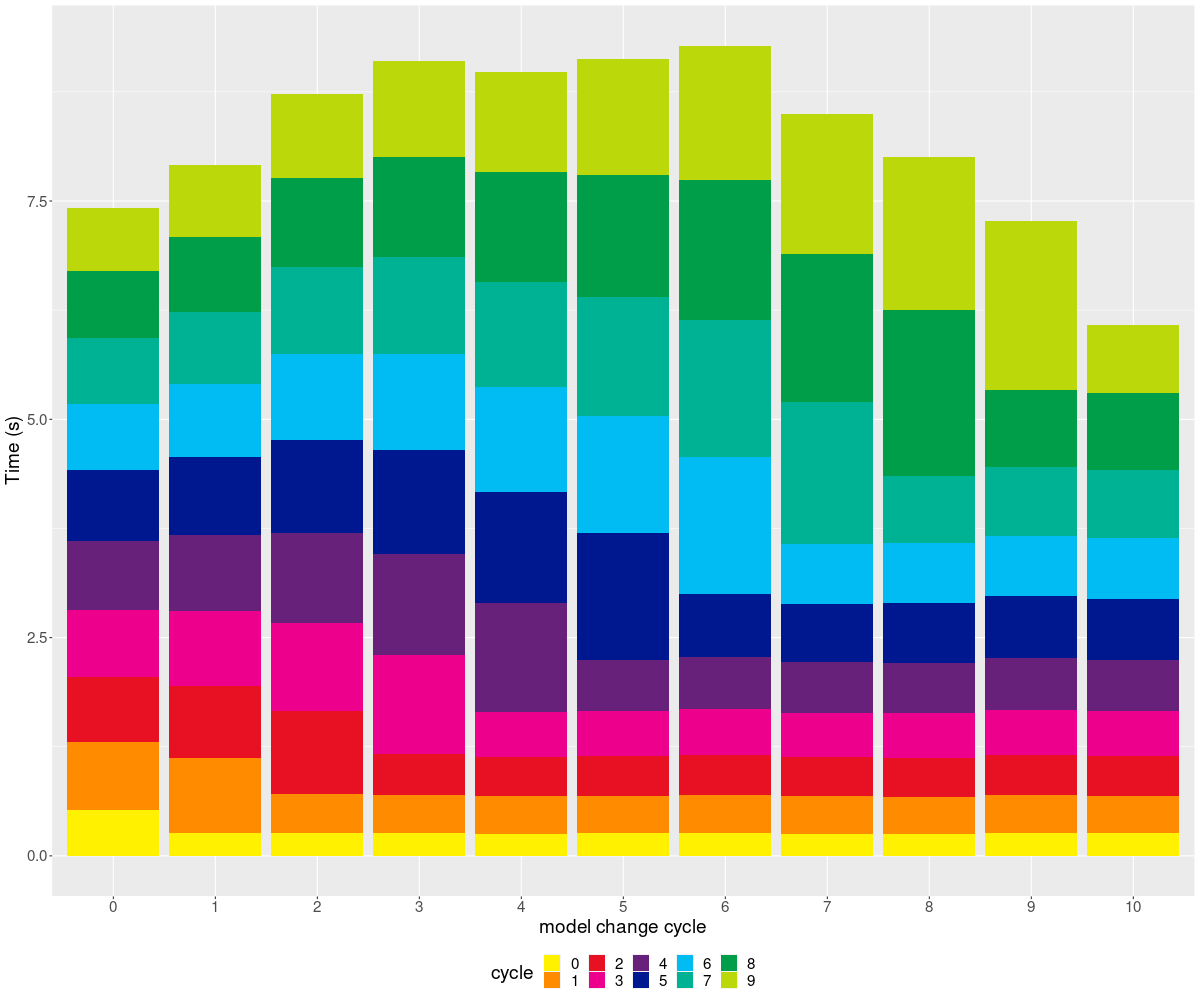
\includegraphics[width=.91\textwidth]{6_model_change/Quicksilver/cycle_log_wallclock_10000particles_8tasks_1ppn.png}
    \caption{Performance of Quicksilver's simulation on 8 MPI ranks,  10,000 input particles}
    \label{fig:6_model_change:quicksilver_8tasks_1ppn_perf}

    \centering
    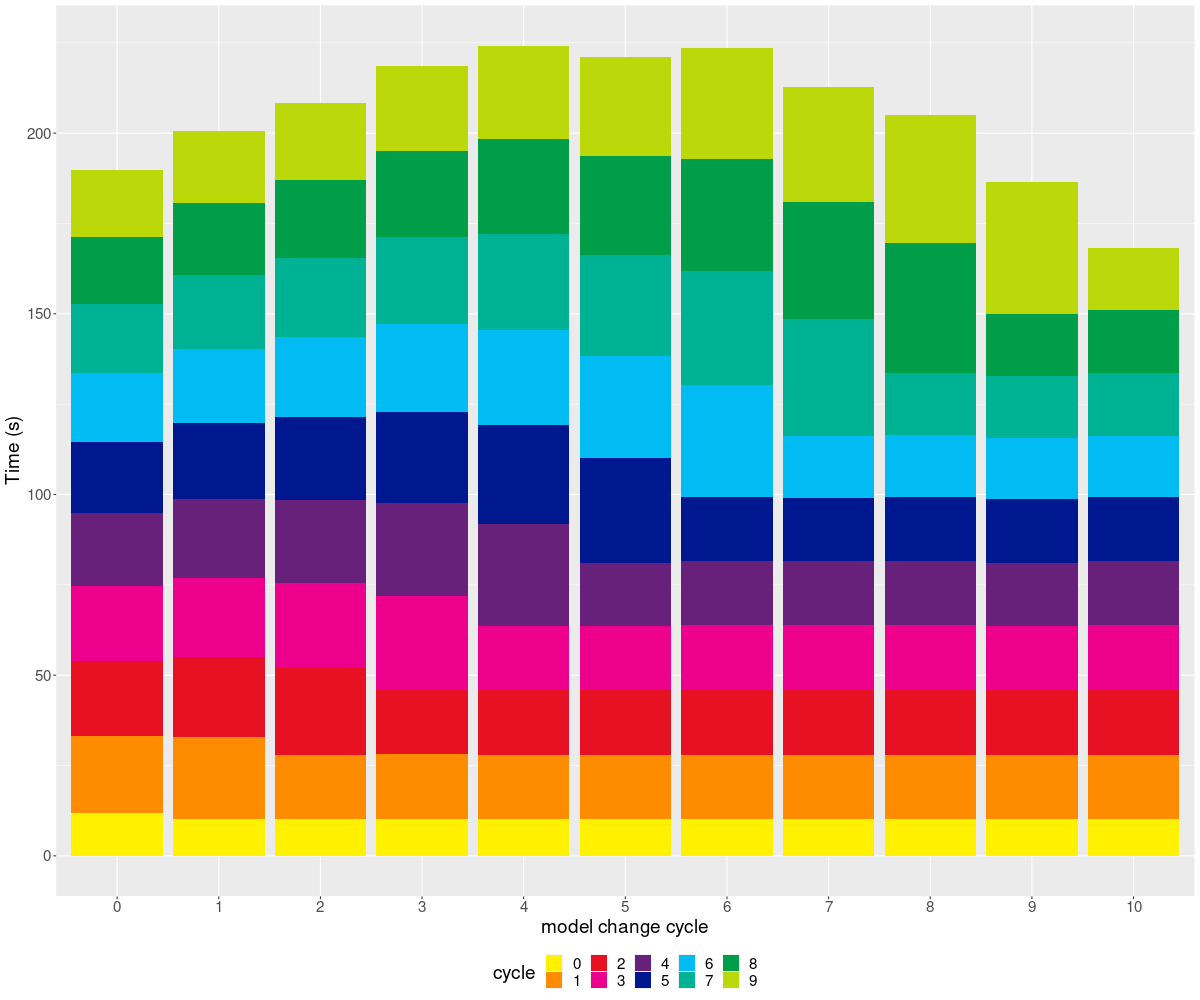
\includegraphics[width=.91\textwidth]{6_model_change/Quicksilver/cycle_log_wallclock_1000000particles_8tasks_1ppn.png}
    \caption{Performance of Quicksilver's simulation on 8 MPI ranks,  1,000,000 input particles}
    \label{fig:6_model_change:quicksilver_8tasks_1ppn_perf_big}
\end{figure}

However, for simulations of more than eight MPI ranks, the performance follows a
very unexpected pattern. This is depicted on
Figure~\ref{fig:6_model_change:quicksilver_8tasks_1ppn_perf}, with simulations
on eight nodes and one process per node: we can see that the performance of the
simulation is the worst when we switch models after cycle number five. In other
words, it is faster to perform a simulation exclusively with our approach,
rather than using SMPI for the first half. If we look at the performance of each
cycle individually, we can see that the first cycles (lower on the bars) always
have the expected duration: they are slow when performed with OpenMPI over
S4BXI, and quicker when performed with SMPI. On the other hand, later cycles
have a completely unexpected performance, as it seems that running SMPI at first
slows down the later cycles (although each cycle should be independent, at least
from the point of view of communications). Although this change in behavior
reminds us of the performance loss of SMPI as the number of MPI ranks increases,
it is a distinct phenomenon: indeed, it always happens around the same number of
MPI ranks, and it does not vary with the problem size. We can confirm this on
Figure~\ref{fig:6_model_change:quicksilver_8tasks_1ppn_perf_big}, where the same
simulations are executed, but with 1,000,000 input particles.

\begin{figure}[!ht]
    \centering
    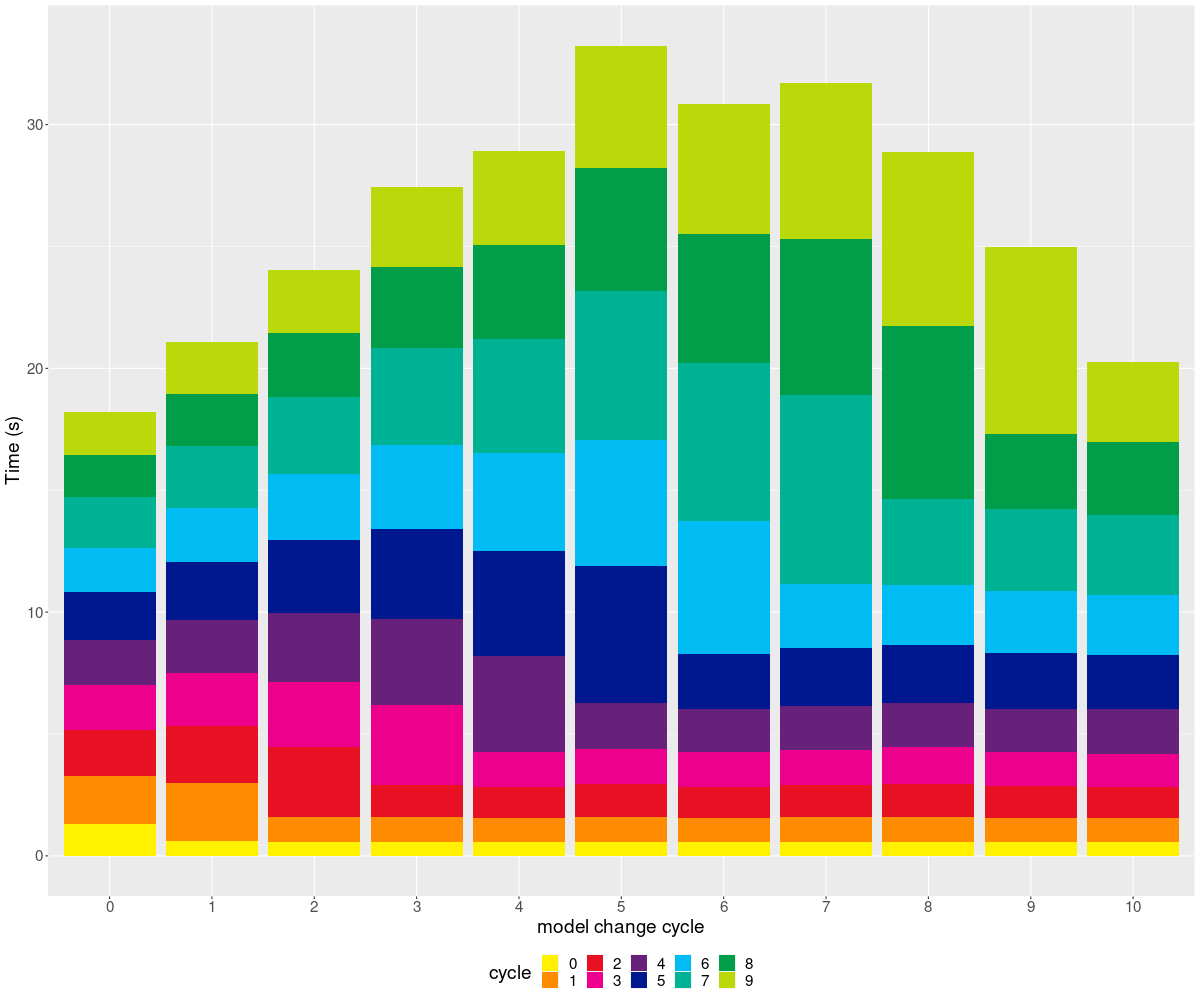
\includegraphics[width=\textwidth]{6_model_change/Quicksilver/cycle_log_wallclock_10000particles_16tasks_1ppn.png}
    \caption{Performance of Quicksilver's simulation on 16 MPI ranks, with 10,000 input particles}
    \label{fig:6_model_change:quicksilver_16tasks_1ppn_perf}
\end{figure}

Finally, we can see on
Figure~\ref{fig:6_model_change:quicksilver_16tasks_1ppn_perf} that this oddity
in our performance measurements only gets worse as we increase the number of MPI
ranks: the figure depicts runs on 16 nodes and one process per node. It gets
even worse since we can see that a simulation which uses only our approach is
faster than a simulation with only SMPI. This confirms that Quicksilver is
particularly pathologic for SMPI, for a reason that we still do not know, even
after running thousands of simulations. Indeed, our analysis of performance
(using Linux's \inline{perf}
tool\footnote{\url{https://github.com/torvalds/linux/tree/master/tools/perf}})
reveals that a large amount of time is spent in SimGrid's code, but it is not
trivial to retrace the calls that might have caused this behavior in SMPI, S4BXI
or users' applications, since Actors issue ``simcalls'' that are then executed
in an entirely different context by SimGrid.

\section{Concluding remarks}
\label{sec:6_model_change:conclusion}

All of these experiments, on OSU micro-benchmarks and Quicksilver, show several
results: first, our model changes behave as expected in many situations.
However, as we have seen, there are several configurations in which our results
are unexpected, and model changes do not help performance at all (in the worst
case it can even lower the performance of simulations). This shows that making
our simulation method more and more complex also makes it more unpredictable,
which is what we wanted to avoid in the first place, by making simulations
instead of real-world experiments. Additionally, we can see that even in
favorable cases, the difference in performance between an experiment fully on
SMPI and fully on OpenMPI is not large enough to make model changes really
useful. Even though switching models can speed up simulations, the order of
magnitude of the execution time is similar, and therefore it will not be
sufficient to model clusters of a very different scale, at least in the current
state of our development. 

Overall, our work shows that dynamic model changes are achievable without
modifying any of the two MPI implementations involved. However, to make them
more useful it would be beneficial to use two models with a more important
difference in performance. For example, we could use an MPI implementation more
simplistic than SMPI, or a very detailed emulator instead of OpenMPI over S4BXI.
Therefore, we believe that our work provides a good framework, which could be
built upon to create simulators with a flexible performance / accuracy tradeoff.
